
% Bug: automatically loads natbib with name options, cannot be
% overridden, `Elsevier LaTeX' style produces error messages

\documentclass[review]{elsarticle}
%\documentclass{elsarticle}

\usepackage{hyperref}
\usepackage{lineno,hyperref} \modulolinenumbers[5]
\usepackage{graphicx}
\usepackage{mathtools}
\usepackage{units}
\usepackage[ruled,vlined]{algorithm2e}
\usepackage{physics} % normal derivative v=dv{x}{t},
                     % partial derivative pdv{V(x,t)}{t}
                     % n'th normal derivative a=dv[2]{x}{t}


\usepackage{color}
\providecommand{\red}[1]{\textcolor{red}{#1}}
\providecommand{\blue}[1]{\textcolor{blue}{#1}}
\definecolor{green}{rgb}{0,0.7,0}
\providecommand{\green}[1]{\textcolor{green}{#1}}

% local macros

%\providecommand{\martin}[1]{\red{#1}} %literal, Preprint
%\providecommand{\martinc}[1]{\green{[#1]}} %comment, Preprint
\providecommand{\martin}[1]{#1}                  %fuer Veroeffentlichung
\providecommand{\martinc}[1]{}                  %fuer Veroeffentlichung

\providecommand{\sup}[1]{^{\mathrm{#1}}}  % upright superscript
\providecommand{\sub}[1]{_{\mathrm{#1}}}  % upright subscript $b\sub{comf}$
                                        % symbolic subscripts without:
                                        % $\epsilon_t$
\providecommand{\3}{{\ss}}

\journal{Transportation Research Part C}

%%%%%%%%%%%%%%%%%%%%%%%
%% Elsevier bibliography styles
%%%%%%%%%%%%%%%%%%%%%%%
%% To change the style, put a % in front of the second line of the current style and
%% remove the % from the second line of the style you would like to use.
%%%%%%%%%%%%%%%%%%%%%%%

%% Numbered
\bibliographystyle{model1-num-names}

%% Numbered without titles
%\bibliographystyle{model1a-num-names}
 
%% Harvard
%\bibliographystyle{model2-names.bst}\biboptions{authoryear}

%% Vancouver numbered
%\usepackage{numcompress}\bibliographystyle{model3-num-names}

%% Vancouver name/year
%\usepackage{numcompress}\bibliographystyle{model4-names}\biboptions{authoryear}

%% APA style
%\bibliographystyle{model5-names}\biboptions{authoryear}

%% AMA style
%\usepackage{numcompress}\bibliographystyle{model6-num-names}

%% `Elsevier LaTeX' style
% \bibliographystyle{elsarticle-num}
%%%%%%%%%%%%%%%%%%%%%%%

\begin{document}

\begin{frontmatter}

\title{Formulation and validation of a car-following model based on deep
  reinforcement learning}

%% Group authors per affiliation:
%\author{Fabian Hart\fnref{myfootnote}}
%\address{TU Dresden}
%\fntext[myfootnote]{Comment.}

%% or include affiliations in footnotes:
\author[firstAddress]{Fabian Hart}
\author[firstAddress,secondAddress]{Ostap Okhrin}
\author[firstAddress,secondAddress]{Martin Treiber\corref{corrAuthor}}
\cortext[corrAuthor]{Corresponding author}
\ead{Martin.treiber@tu-dresden.de}
\ead[url]{www.mtreiber.de}

\address[firstAddress]{TU Dresden}
\address[secondAddress]{Possible second address}




\begin{abstract}
\martinc{After the final research has settled, I can write it}
\end{abstract}

\begin{keyword}
reinforcement learning \sep car-following model \sep stochastic
processes \sep string stability \sep validation \sep trajectory data 
\end{keyword}

\end{frontmatter}

%\linenumbers

\section{Introduction}
Autonomous driving technologies are seen as promising solutions to
improve road safety, where human errors account for 94\% of the total
accidents \citep{vehicleCrashSurvey2015}.  
\martinc{Das ``author'' Attribut in Bibtex darf man nicht
  fuer anderes missbrauchen, da je nach Zitierstil nur zwei Autoren
  drankommen und bibtex diverse andere Manipulationen vornimmt; .bib
  File korrigiert.}
  \martinc{citep=cite with parentheses}
Moreover, congestion, energy
consumption, and emissions \martinc{Die Englaender haben bei
  Aufzaehlungen von $\ge 3$ items auch vor dem ``and'' ein Komma} are intended to be reduced. 
\martin{On the other hand,} autonomous driving is a challenging task
since \martin{traffic flow} can be dynamic and unpredictable.
On the way to fully autonomous driving, Advanced Driver Assistance Systems
(ADAS) have been developed to solve tasks like car following, emergency
braking, lane keeping, or lane changing. \martinc{``like'' startet
  bereits eine unvollst\"andige Aufz\"ahlung, so no need for ``etc.''}
\martinc{Bindestriche in zusammengesetzten Worten gibt es i.A. nur bei 
  $\ge 3$ Teilen, und zwar in alle L\"ucken au\3er der letzten, also
  \emph{lane changing} aber \emph{lane-changing model}}
Since Deep Learning methods have been demonstrated to surpass humans
in certain domains, they are also adopted in the area of autonomous
driving.
\martinc{Generelles ueber which vs. that: 
1. \emph{which mit Komma:}
  ``non-defining clauses'': der darauf folgende Relativsatz gibt interessante Details,
  schraenkt das Subjekt/Objekt im Hauptsatz aber nicht ein (I use my bike, which has 18
  gears, rather often)
2. \emph{which ohne Komma oder besser ``that'' oder ein Gerund (``ing-Form''):} ``defining clauses''. Der darauf folgende Relativsatz enthaelt einschraenkende,
wesentliche Informationen: ``The bike that/which has a
broken chain/having a broken chain is in the garage'' (impliziert,
dass ich mindestens ein zweites Rad habe). Im Folgenden ist eine ``nice-to
mention''-Definition, also ist which mit Komma OK, oft folgen bei dir dann
aber defining clauses, die ich durch ``that'', ``who'' (bei Menschen)
oder einem Gerund ersetzt habe. Pedantische Korrewktoren nennen das
auch ``which hunting'' (witch=Hexe)}
Especially Deep Reinforcement Learning (DRL), which combines the power
using deep neural networks with Reinforcement Learning, has shown its potential in a broad variety of autonomous driving tasks. 
In \cite{OnRampMerge2018} and \cite{OnRampMerge2020}, DRL is used to
guide an autonomous vehicle safely via an on-ramp to the freeway. In \cite{intersection1}, \cite{intersection3} and \cite{intersection2}, DRL methods are used to manage traffic of autonomous vehicles at intersections, optimizing safety and efficiency.
In \cite{LangeChange1}, DRL is used to solve lane-changing maneuvers.

A further task in autonomous driving is to model the vehicle behavior
under car-following scenarios, where suitable accelerations has to be
computed in order to achieve safe and comfortable driving. Approaches
for solving this task are classical car-following models, such as the
Intelligent Driver Model \citep{Opus} or stochastic car-following
models \martin{such as that of} \cite{Treiber2018stochIDM_TRB}. Furthermore, data-driven approaches used Machine Learning methods to train a car-following model based on experimental car-follower data, such as in \cite{Chong2011SimulationOD} or \cite{ZHOU2017245}. The downside of this approach is that the model tries to emulate human driver behavior, which can still be suboptimal.

To overcome this issue, DRL methods train non-human car-following models that can optimize metrics such as safety, efficiency, and comfort. 
One approach is to train on scenarios where the leading vehicle
trajectory, used for training, is based on experimental data, such as
in \cite{SafeEfficientAndComfortable} or
\cite{HumanLikeAutonomouCF}. Similar approaches suggest a standardized
driving cycle \martin{serving as a} leading vehicle trajectory, such
as \cite{ComparisonRLvsMPC} or \cite{CFelectricVehicle}
\martin{who}\martinc{relative clauses mit Menschen: ``who'' statt
  ``which'' oder ``that''} use the New European Driving Cycle.
A disadvantage coming along with these approaches is that the
performance decreases for scenarios \martin{that} are not in the scope of the training data, indicating inadequate machine learning generalization \citep{ComparisonRLvsMPC}. 

Another issue of car-following models is string stability. There are
several studies focusing on dampening traffic oscillations by using a
sequence of trained vehicles, such as these by \cite{qu2020jointly}, \cite{DissipatingStopAndGoWaves}, and \cite{DampenStopAndGoTraffic}.

All the mentioned DRL car-following models have three disadvantages in
common: First, the acceleration range is limited in a way that
full-braking maneuvers are not considered. This results in models that are just designed for non-safety-critical scenarios. Second, these models just consider car-following scenarios, while free driving or the transition between both is not reflected in the reward function. Third, the trained models have just been validated on data that is similar to the training data set so that the generalization capabilities cannot be proven. 

This motivated us to design a model \martin{that} overcomes these issues.
To our knowledge, no RL based car-following model has been proposed \martin{that} has the following features combined:


\begin{itemize}
	\item  The proposed model considers free driving,
          car-following, as well as the transition between both in a
          way that approaching the leading vehicle is \martin{always} smooth and comfortable.
	\item The proposed model has a wider range of possible
          accelerations \martin{leading} to a collision-free behavior
          also in safety-critical situations such as a full-braking maneuver of the leader.
	\item The proposed model is trained on leading trajectories,
          based on an AR(1)-process (see, e. g., \cite{HonerkampEngl})
          with parameters reflecting the kinematics of real
          drivers. This leads to high generalization capabilities and
          model usage in a broader variety of traffic
          scenarios. \martin{Moreover, the supply of learning data is
            unlimited.} 
	\item Different driver characteristics can be modeled by adjusting the parameters of the reward function.
	\item The proposed model shows string stability \martin{even in
          extreme situations}.
	
\end{itemize}

Another feature of this work is a thorough validation of the above-mentioned properties in scenarios based on both synthetic and real trajectory data, bringing the model to its limits. 
In all cases, the model proved to be accident-free and string stable.
In a further experiment, the proposed model is compared to the Intelligent Driver Model calibrated on the same data. The results indicate a better performance of the proposed model.

\martinc{Nach vorgestelltem Nebensatz oder Phrase (In Section ...,) folgt vor dem
  Hauptsatz (``we introduce...'') immer ein Komma}
This work is structured as follows. In Section \ref{sec:RLBackground},
we introduce some basic RL background as well as our modularized RL
approach, followed by a detailed description of our two sub-modules:
the Free-Driving policy in Section \ref{sec:FreeDrivingPolicy} and the
Car-Following policy in Section
\ref{sec:CarFollowingPolicy}. \martinc{In Englisch wird nach
  Doppelpunkt klein weitergeschrieben, wenn kein vollst\"andiger Satz
  folgt wie hier} In Section \ref{sec:validation}, we evaluate our RL
strategy with respect to safety, \emph{stability}, and comfort aspects
before we conclude in Section \ref{sec:conclusion}.


\section{Reinforcement Learning Background}
\label{sec:RLBackground}

The \martin{follower} is controlled by a Reinforcement
Learning (RL) agent. By interaction with an environment, the RL agent
optimizes a sequential decision-making problem. At each time step
$t$, the agent observes an environment state $s_t$ and, based on that state, selects
an action $a_t$. After conducting action $a_t$, the RL agent receives
a reward $r(a_t,s_t)$. The agent aims to learn an optimal state-action
mapping policy $\pi$ that maximizes the expected accumulated
discounted reward
\begin{equation}
\label{Rt}
R_{t}=\sum_{k=0}^{\infty} \gamma^{k} r_{t+k},
\end{equation}
 where $\gamma = (0,1]$ denotes the discount factor and 
$\gamma^k r_{t+k}$ the expected contribution $k$ time steps ahead. 
  \subsection{\label{RL-algorithm}RL algorithm}
  In various similar control problems, the Deep Deterministic Policy
  Gradient (DDPG) Algorithm has been used and proven to perform well on
  tasks with a \martin{deterministic and} continuous action and a
  continuous state space, such as in
  \cite{SafeEfficientAndComfortable}, \cite{ComparisonRLvsMPC} or
  \cite{HumanLikeAutonomouCF}. The original work can be found in
  \cite{DDPG}. DDPG is an actor-critic method, that uses an actor
  $\mu\left(s \mid \theta^{\mu}\right)$ with weights $\theta^{\mu} $
  to propose an action based on a given state $s$ and a critic
  $Q\left(s, a \mid \theta^{Q}\right) $ with weights  $\theta^{Q}$ to
  predict if the action is good or bad, based on a given state $s$ and
  action $a$. \martinc{Ich w\"urde Subskripte f\"ur die Parameter(vektoren?)
  $\theta_{\mu}$ und $\theta_Q$ nehmen. Oder sind die Superskripte
    Konvention hier?}
\martinc{Ferner ist mir nicht klar, wie sich die
    Einleitung (Parameter des Aktions-Algorithmus bzw  Policy $\pi$ so w\"ahlen, dass der reward $R_t$
    maximiert wird) von der
    Actor-Critic Darstellung unterscheiden. F\"ur mich ist der Actor
    $\mu|\theta$ einfach der Algorithmus $\pi|\theta$ und die Critic die
    Rewardfunktion $R_t$, die als kumulierter Reward eigentlich keine im Lernprozess
    ver\"anderbaren Parameter hat, also alter Wein in neuen
    Schl\"auchen: Der Unterschied zu bzw. die Pr\"azisierung der
    Einleitung sollte klar werden, Au\3erdem, dass $\theta$ wohl den
    Vektor der Synapsenst\"arken/Linkst\"arken des jeweiligen NN angibt.)} 
To achieve a better training stability, DDPG uses target networks  $\mu^{\prime}$ and $Q^{\prime}$ for actor and Critic. While training, these networks are updated slowly, hence keeping the estimated targets stable. Furthermore DDPG uses Experience Replay, that implements a Replay Buffer $R$, where a list of tuples $\left(s_{t}, a_{t}, r_{t}, s_{t+1}\right)$ are stored. Instead of learning from the most recent experience, DDPG learns from sampling a mini-batch from the experience buffer. To implement better exploration by the actor network, DDPG uses noisy perturbations, specifically an Ornstein-Uhlenbeck process for generating noise. It samples noise from a correlated normal distribution. The entire DDPG algorithm is shown in Algorithm~\ref{alg:ddpg}. 
  
  \begin{algorithm}
  	\label{alg:ddpg}
  	Randomly initialize critic network $Q\left(s, a \mid \theta^{Q}\right) $ and actor $\mu\left(s \mid \theta^{\mu}\right)$ with weights $\theta^{Q}$ and $\theta^{\mu} $  \\
  	Initialize target network $Q^{\prime}$ and $\mu^{\prime}$ with weights $\theta^{Q^{\prime}} \leftarrow \theta^{Q}, \theta^{\mu^{\prime}} \leftarrow \theta^{\mu}$\\
  	Initialize Replay Buffer $R$\\
  	\For{$episode = 1$ \KwTo $M$}{
  		Initialize a random process $\mathcal{N}$ for action exploration\\
  		 Receive initial observation state $s_{1}$ \\
  		\For{$t = 1$ \KwTo $T$}{
  			Select action $a_{t}=\mu\left(s_{t} \mid \theta^{\mu}\right)+\mathcal{N}_{t}$ according to the current policy and exploration noise\\
  			 Execute action $a_{t}$ and observe reward $r_{t}$ and observe new state $s_{t+1}$\\
  			  Store transition $\left(s_{t}, a_{t}, r_{t}, s_{t+1}\right)$ in $R$\\
  			   Sample a random minibatch of $N$ transitions $\left(s_{i}, a_{i}, r_{i}, s_{i+1}\right)$ from $R$\\
  			    Set $y_{i}=r_{i}+\gamma Q^{\prime}\left(s_{i+1}, \mu^{\prime}\left(s_{i+1} \mid \theta^{\mu^{\prime}}\right) \mid \theta^{Q^{\prime}}\right)$\\
  			Update critic by minimizing the loss:
                        \martinc{Ich dachte, der/die Critic ist der feste
                          Qualit\"atsgutachter und der Actor wird an
                          die Critic angepasst. Wird hier wirklich
                          umgekehrt die
                          Critic angepasst? (``Ich habe
                          danebengeschossen. Lasst uns die Zielscheibe
                          dorthin versetzen, wohin ich geschossen habe'')}  $L=\frac{1}{N} \sum_{i}\left(y_{i}-Q\left(s_{i}, a_{i} \mid \theta^{Q}\right)\right)^{2}$\\
  			 Update the actor policy using the sampled policy gradient:
  			$$
  			\left.\left.\nabla_{\theta^{\mu}} J \approx \frac{1}{N} \sum_{i} \nabla_{a} Q\left(s, a \mid \theta^{Q}\right)\right|_{s=s_{i}, a=\mu\left(s_{i}\right)} \nabla_{\theta^{\mu}} \mu\left(s \mid \theta^{\mu}\right)\right|_{s_{i}}
  			$$
  			Update the target networks:
  			$$
  			\begin{aligned}
  			\theta^{Q^{\prime}} & \leftarrow \tau \theta^{Q}+(1-\tau) \theta^{Q^{\prime}} \\
  			\theta^{\mu^{\prime}} & \leftarrow \tau \theta^{\mu}+(1-\tau) \theta^{\mu^{\prime}}
  			\end{aligned}
  			$$
  		}
  	}
  	
  	
  	\caption{DDPG algorithm according to \cite{DDPG}}
  \end{algorithm}
  
  
  \subsection{\label{MRL}Modularized Reinforcement Learning}
  Furthermore we used a modularized approach to decompose the task into two subtasks. Modular Reinforcement Learning (MRL) refers to the decomposition of a complex, multi-goal
  problem into a collection of simultaneously running single goal learning processes, typically modeled as Markov Decision Processes. Typically, these subagents share an action
  set but have their own reward signal and state space. At each
  time step, every subagent reports a numerical preference for
  each available action to an arbitrator which then selects one
  of the actions for the agent as a whole to take (\cite{MRL}). There are numerous works, that are using a modularized Reinforcement Learning approach, like in \cite{MRLexample1}, \cite{MRLexample2} or \cite{MRLexample3} just to name a few. The advantage of decomposing multiple-goal reward functions with MRL, we also want to use in this work. 
  Figure \ref{fig:MRL} shows the architecture of our MRL System. We divide our car-following problem into two subtasks, handled by two different policies. The Free-Driving Policy refers to free driving and aims to not to exceed a desired speed. The Car-Following Policy refers to following a vehicle and aims to keep a reasonable gap to a leader vehicle. Although both policies are trained with different reward functions and in different training environments, they both output an acceleration value. As an arbitrator between both accelerations we use a simple min-function. We adopted this approach from the IDM+, that also uses separate terms for free-flow and interaction with a leading vehicle (\cite{idm_plus}). In the next sections the model specifications of the Free-Driving Policy and the Car-Following Policy, which are both trained with the DDPG algorithm, are described in detail.
  
  \begin{figure}
  	\centering
  	\includegraphics[width=12cm]{images/MRL_small}
  	\caption{Modularized RL architecture with actor networks of both policies.} 
  	\label{fig:MRL}
  \end{figure}

  
  % In this study, both networks are feed-forward neural networks with two layers of hidden neurons and %32 neurons each hidden layer. All DDPG parameters are presented in Table \ref{tab:DDPGparameters}.
  



\section{Free-Driving Policy}
\label{sec:FreeDrivingPolicy}
\subsection{Action and state space}
\label{stateSpaceFree}
 The defined modularized RL approach requires that the action space of
 both sub-policies are identical. \martin{In our use case, the action space is
 continuous and one-dimentional and given by the range of feasible accelerations
 $\dot{v}_t \in [a\sub{min}, a\sub{max}]$. The range limits
 $a\sub{min}= \unit[-9]{m/s^2}$ and  $a\sub{max} =\unit[2]{m/s^2}$
 reflect comfortable driving ($\dot{v}_t \le a\sub{max}$) while
 allowing for the physical limit $-a\sub{min}$ of the braking
 deceleration} in safety-critical
situations

The state space defines the observations that the 
vehicle can receive from the environment. To compute an optimal
acceleration, the following vehicle observes its own acceleration $\dot{v}$,
and its own speed $v$. Linear translation and scaling is used to
reduce the dimensions and to bring all observations approximately into
the same range of $[0,1]$. The observation \martin{vector} at time step $t$ is defined
as 

\begin{equation}
\label{eq:stateFree}
s_t = \begin{pmatrix} \frac{v_t}{v\sub{des}} \\ \frac{\martin{\dot{v}}_t-a\sub{\rm min}}{a\sub{\rm max} - a\sub{\rm min}}\end{pmatrix}.
\end{equation}
\subsection{Reward Function}
\label{rewardFunctionFree}
The reward function contribution a time step $t$ is decomposed into two factors. The first part aims to
not exceed a desired speed $v\sub{des}$, but also to accelerate if the
desired speed is not reached yet.  
\martinc{Man sollte auch den Fall $v>v\sub{des}$ ber\"ucksichtigen,
  der z.B. durch Einfahren in ein Streckensegment mit niedrigerem
  Tempolimit (Ortseinfahrt) realisiert wird, aber nicht so
  drastisch/unstetig wie hier, z.B. zweiten Fall durch
  $(v\sub{des}-v)/v\sub{des}$ statt =0 ersetzen}

\begin{equation}
\label{eq:r1Free}
	r_1  = 
	\begin{cases}
	\frac{v}{v\sub{des}},
	& \text{if } v < v\sub{des}\\
	0
	 & \text{otherwise}
	\end{cases}
\end{equation}

The second part of the reward function aims to reduce the jerk in
order to achieve comfortable driving, \martinc{No need for dotted
  quantities here; I propose using $j\sub{comf}$} \martinc{Really
  $\dv{a}{t}$ or the second state variable defined in~\eqref{eq:stateFree}?}
\begin{equation}
\label{eq:r2Free}
r_2 = -\left(\frac{1}{j\sub{comf}} \ \dv{a}{t}\right)^2.
\end{equation}
%
Since building up a comfortable value of acceleration or deceleration
from zero in one second is at the limit of comfortable jerks, $r_2$
values above unity tend to feel uncomfortable.


The contribution of the final reward function at simulation time step $t$ is the weighted
sum of these factors according to
\begin{equation}
\label{rt1}
r_t =r_1 + w\sub{jerk} r_2,
\end{equation}
where all the factors are evaluated at time step $t$. 


\subsection{Training environment}
\label{training_environment1}
In order to train the RL agent for the task of keeping a desired
speed, the training environment is defined as follows. To describe the
dynamics of the vehicle, a point-mass kinematic model is used. For
updating the speed and position for time step $t + 1$ the Euler and
ballistic methods are used, respectively. This approach is recommended in \cite{numericalUpdateMethodsTreiber} as an efficient
and robust scheme for integrating car-following models.

\begin{equation}
	v_{t+1} = v_{t} + \martin{\dot{v}_{t}} d
\end{equation}

\begin{equation}
x_{t+1} = x_{t} + \frac{v_{t} + v_{t+1}}{2} d
\end{equation}


with $d$ corresponding to the simulation step size \martin{that} is globally
set to \unit[100]{ms}. To train the RL agent, a training episode has to be defined. One training episode contains 500 time steps and the vehicle's initial speed is set randomly in the range $[0,v\sub{des}]$.

\subsection{Model training}
Both neural networks, critic and actor, are feed-forward neural
networks with one layer of hidden neurons, containing 16 neurons (see
Figure \ref{fig:MRL}). ReLU activation functions (\cite{relu}) are used. The learning rate for
critic and actor is set to 0.001. \martinc{Ist das die Variable $\tau$
  in Algorithm~1? Bitte kl\"aren} For the exploration of the action
space, an exploration noise model has to be defined. We adopted a
zero-reverting Ornstein-Uhlenbeck process with $\Theta = 0.15$  and
$\sigma = 0.2$ as suggested in
\cite{DDPG}. \martinc{Einheitenbehaftet, also in $\unit[]{m/s^2}$ oder
  ist der action space skaliert gem\"a\3 der 2. Komponente des State
  Vektors?} The soft update rate of the target networks $\tau$ is set to
0.001.\martinc{Och, noch eine Tiefpass-Zeitvariable der Gr\"o\3e
  0.001. Welche von den beiden ist $\tau$?}
All DDPG parameters are presented in Table \ref{tab:DDPGparameters}.
%
  \begin{table}
	\caption{DDPG parameter values} 
	\label{tab:DDPGparameters} 
	\begin{center}
		\begin{tabular}{ p{0.4\textwidth} p{0.2\textwidth}  p{0.2\textwidth} }
			 & Free-Driving Policy & Car-Following Policy \\ \hline
			Learning rate & 0.001 & 0.001\\ 
			Reward discount factor & 0.95 & 0.95 \\ 
			Experience buffer length & 100000 & 100000 \\ 
			Mini batch size & 32 & 32 \\ 			
			Ornstein-Uhlenbeck  $\Theta$ & 0.15& 0.15 \\ 
			Ornstein-Uhlenbeck  $\sigma$ & 0.2 & 0.2 \\ 
			Number of hidden layers & 1 & 2\\
			Neurons per hidden layer & 16 & 32\\
			Soft target update  $\tau$ & 0.001 & 0.001\\
			
			
		\end{tabular}
	\end{center}
\end{table}
%
\martinc{Evtl. diese Abb vorziehen. Manche Journals wollen Bilder in
  der Reihenfolge der ersten Erwaehnung im Haupttext}
Figure \ref{fig:TrainingReward} shows an example of the training
process, where the asymmetric moving average reward of the last 30 training episodes is plotted over training episodes. For the Free-Driving Policy, a maximum average reward has been reached after approximately 3200 training episodes (marked in red).
%
\begin{figure}
	\centering
	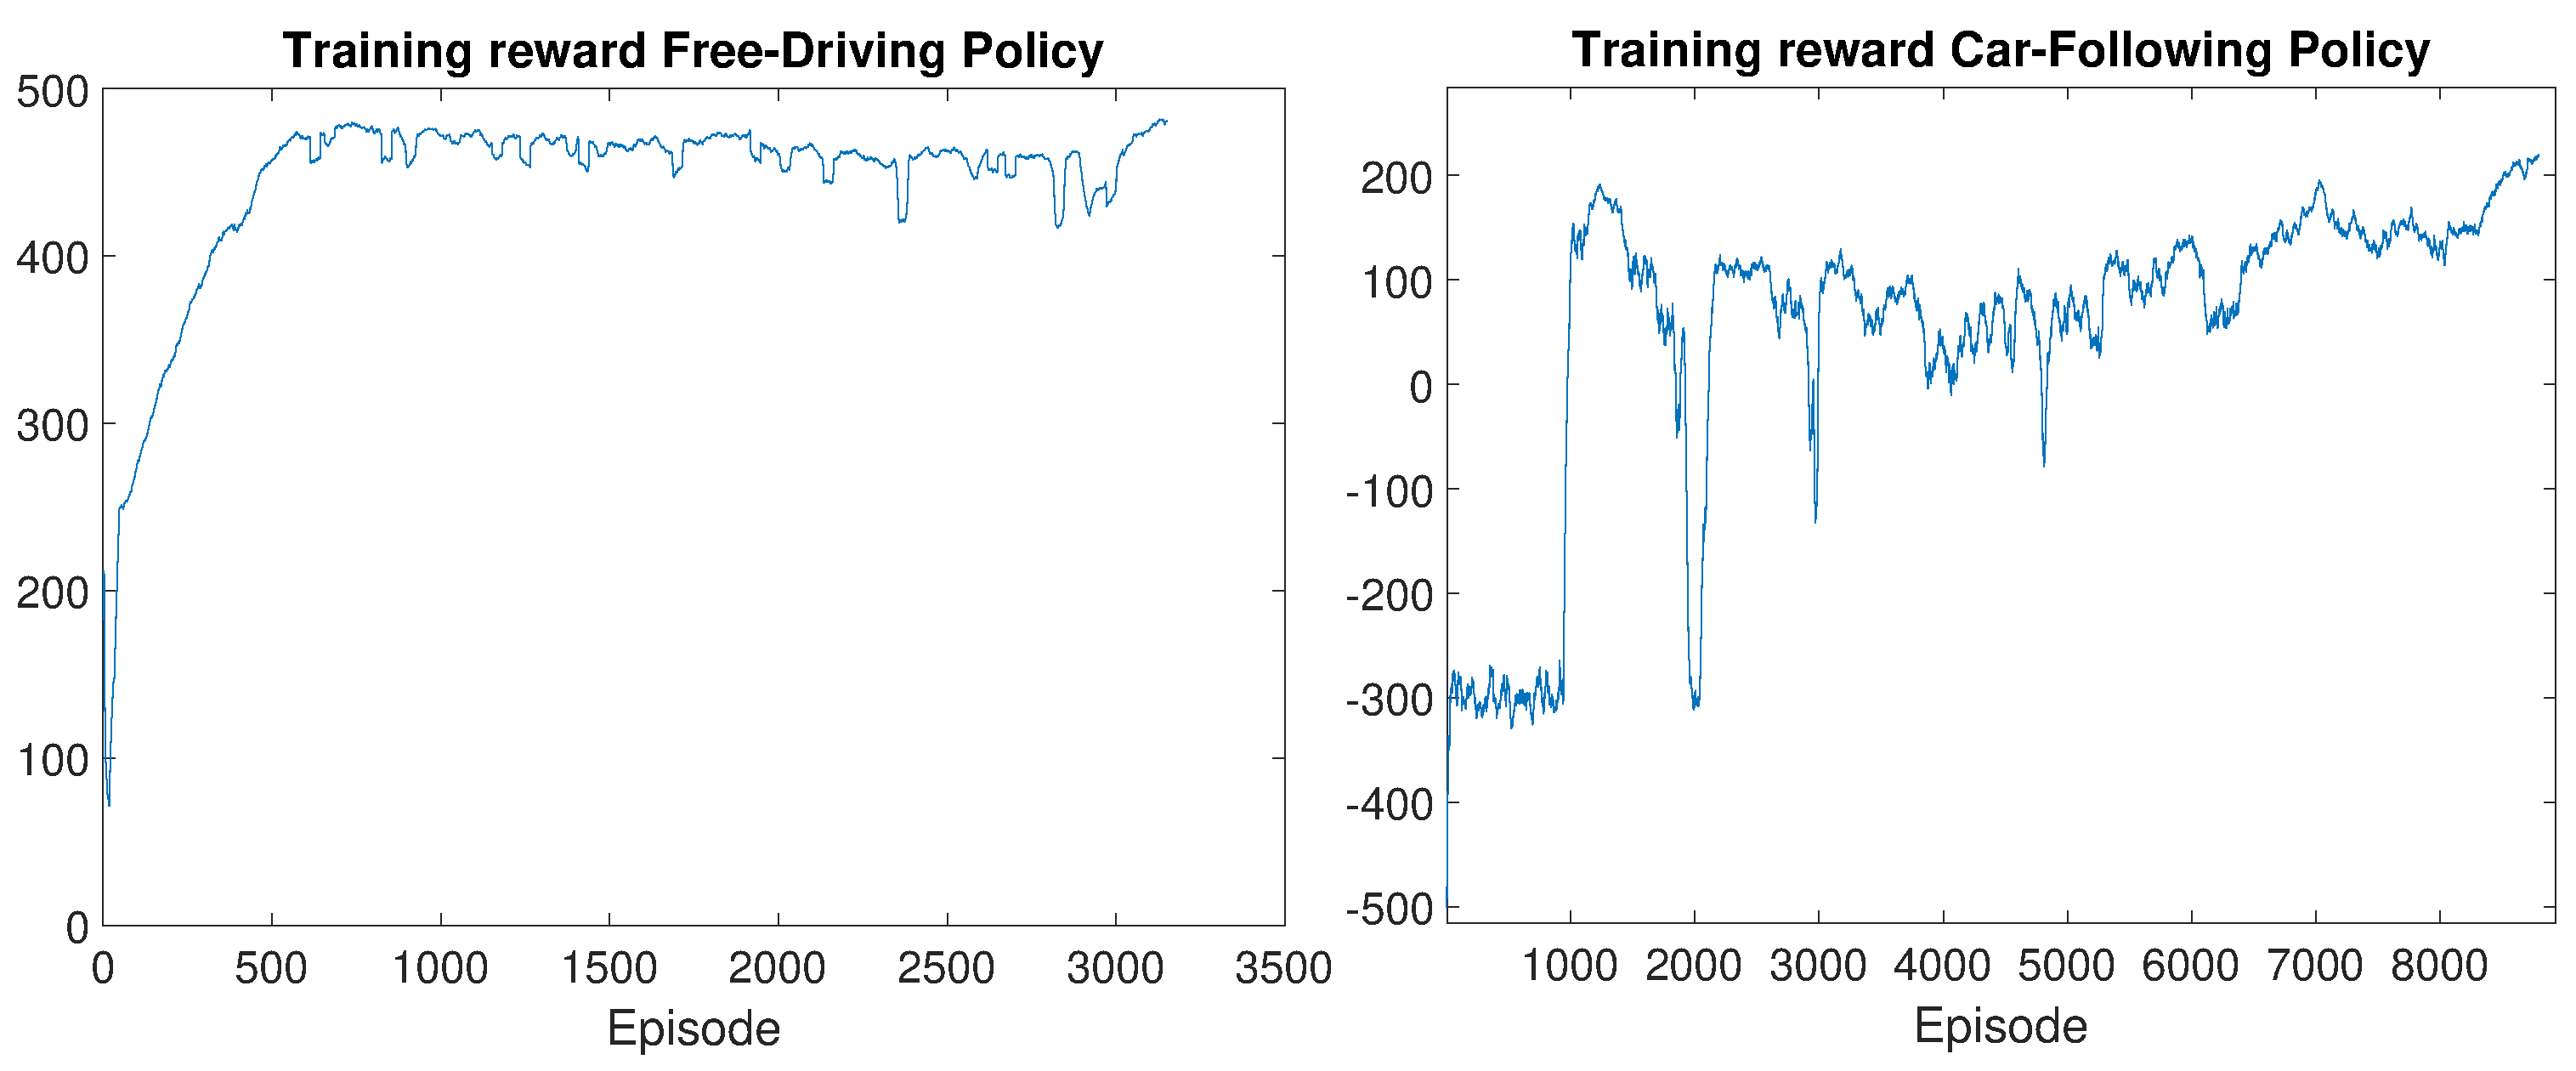
\includegraphics[width=12cm]{images/TrainingReward}
	\caption{Asymmetric moving average reward of the last 30 training episodes for Free-Driving Policy and Car-Following Policy} 
	\label{fig:TrainingReward}
\end{figure}


\section{Car-Following Policy}
\label{sec:CarFollowingPolicy}
\subsection{Action and state space}
\label{stateSpaceFollow}
To match the action space of the Free-Driving Policy, the acceleration is analogously defined as a continuous variable in the range between $a\sub{\rm min} = \unit[-9]{m/s^2}$ and 
$a\sub{\rm max} =\unit[2]{m/s^2}$.


The state space defines the observations that the following
vehicle can receive from the environment. To compute an optimal
acceleration, the following vehicle uses its own acceleration $a$,
its own speed $v$, the leader's speed $v_l$,
and the (bumper-to-bumper) gap $g$.
 Again, linear translation and scaling is used
to reduce the dimensions and to bring all observations approximately
into the same range of $[-1,1]$. The observation at time step $t$ is defined as

\begin{equation}
\label{eq:stateFollow}
s_t = 
\begin{pmatrix} 
\frac{v}{v\sub{des}} \\ 
\frac{\dot{v}-a\sub{\rm min}}{a\sub{\rm max} - a\sub{\rm min}}\\
\frac{v_l-v}{v\sub{des}}\\
\frac{g}{g\sub{\rm max}}

\end{pmatrix},
\end{equation}
%
where $g\sub{max}$ is set to  \unit[200]{m}. When $g$ exceeds  $g\sub{max}$ or there is no leader, $g$ is set to  $g\sub{max}$.

\subsection{Reward Function}
\label{rewardFunctionFollow}
\martinc{Die reward function ist nicht als Funktion des skalierten
  Statevektors S $s_t$, sondern mit Hilfe der unskalierten Statevariablen
  formuliert (obwohl die meisten Terme der Rewardfunktion ihre eigene
  Skalierung enthalten, nicht aber $r_1$). Stimmt das? Falls nicht, h\"atte man das Problem, dass
  in Extremf\"allen (Tempo 130 oder 150 auf stehendes Hindernis)
  $g\sub{max}=\unit[200]{m}$ nicht ausreicht. Ignoriert die reward
  function die skalierten States (warum braucht man die dann aber?),
  gibt es hingegen kein Problem.}
The goal of the Car-Follower-Policy is to reduce the crash risk, while
maintaining comfortable driving in non-safety-critical situations. The
reward function includes a set of parameters that can be
adjusted to realize different driving styles. 

\begin{table}
	\caption{RL agent parameters and default values} 
	\label{tab:agentParameters} 
	\begin{center}
		\begin{tabular}{ p{0.12\textwidth}| p{0.65\textwidth}| p{0.1\textwidth}}
			Parameter & Description & Value \\ \hline
			$a\sub{\rm min}$ & Minimum acceleration & $\unit[-9]{m/s^2}$ \\  
			$a_{\rm max}$ & Maximum acceleration & $\unit[2]{m/s^2}$ \\  
			$b_{\rm comf}$ & Comfortable deceleration & $\unit[2]{m/s^2}$ \\  
			$j_{\rm comf}$ & Comfortable jerk & $\unit[2]{m/s^3}$ \\  
			$v_{\rm des}$ & Desired speed & $\unit[15]{ m/s}$ \\  		
			$T$ & Desired time gap to the leading vehicle & $\unit[1.5]{s}$ \\
			$g_{\rm min}$ & Desired minimum space gap & $\unit[2]{m}$ \\
			$T_{\rm lim}$ & Upper time gap limit for zero reward (see
			Eq. \eqref{eq:r1Free}) & $\unit[15]{s}$ \\
			$w\sub{gap}$ & relative weight for keeping the desired gap & 0.5\\
			$w\sub{jerk}$ & relative weight for comfortable acceleration & 0.004\\
		\end{tabular}
	\end{center}
\end{table}



The reward function contribution at time step $t$ consists of three factors. 
The first factor addresses the driver's
response in safety-critical situations by comparing the
kinematically needed deceleration (assuming an
unchanged speed of the leader) with the
comfortable deceleration $b\sub{comf}$,



\begin{equation}
\label{eq:r1_CFP}
r_1 = 
\begin{cases}
-\tanh\left(\frac{b_{kin}-b\sub{comf}}{-a\sub{min}}\right),& \text{if } b_{kin}>b\sub{comf}\\
0,              & \text{otherwise}
\end{cases}
\end{equation}

with
\begin{equation}
\label{bkin}
b_{kin} = 
\begin{cases}
\frac{(v-v_l)^2}{g},& \text{if } v>v_l\\
0,              & \text{otherwise}
\end{cases}
\end{equation}
The argument of the tanh function with  the
maximum possible deceleration ($\approx \unit[9]{m/s^2}$ on dry roads) gives a
non-dimensional measure for the seriousness of the critical situation
with values 
near or above 1 indicating an imminent crash.  The tanh function functions as a limitation for the reward value to the range [-1,0]. This has shown to make the learning process more stable. Notice that the case distinction in ~\eqref{eq:r1_CFP}  ensures that
this term is not activated in non-critical situations. The purpose of
the factor $r_1$ is twofold: It motivates the follower vehicle to
brake in safety-critical or near-crash situations.  Furthermore it
motivates the follower vehicle also to brake early in non-critical
situations, where $ v>v_l$, in order to achieve a comfortable
approaching of the leader vehicle.\martinc{Nicht wirklich, weil diese
  Funktion nur in zumindest milde kritischen Situationen $b\sub{kin}>b\sub{comf}$ anspringt.}

The second part of the reward function aims to not fall below a reasonable
distance to the leading vehicle.


\begin{equation}
\label{eq:r2_CFP}
r_2  = 
\begin{cases}
\frac{\varphi((g-g\sub{opt})/g\sub{var})}{\varphi(0)},
& \text{if } g < g^*\\
\frac{\varphi((g-g\sub{opt})/g\sub{var})}{\varphi(0)}
\left(1-\frac{g-g^*}{g\sub{lim} - g^*}\right)  & \text{otherwise}
\end{cases}
\end{equation}
with 
\begin{equation}
\label{eq:r21}
g\sub{opt} = vT + g\sub{min},
\end{equation}
\begin{equation}
\label{eq:r22}
g\sub{var} = 0.5g\sub{opt},
\end{equation}
\begin{equation}
\label{eq:r23}
g\sub{lim} = vT\sub{lim} + 2g\sub{min},
\end{equation}
%
and $\varphi(x)$ describing the standard-normal probability density
function. The value of $g^*$ is chosen in a way, that the reward function $r_2$ is differentiable.
%
\begin{figure}
	\centering
	\includegraphics[width=12cm]{images/RewardFunc1}
	\caption{Factor 2 of the reward function maximizing the reward
		for car following with time gap $T$} 
	\label{fig:RewardFunc1}
\end{figure}
%
Figure \ref{fig:RewardFunc1} illustrates the reward function for
$r_2$, containing the parameter $g\sub{opt}$, $g^*$ and $g_{\rm
	lim}$. The reward function is designed in a way, that for high speeds $v$
of the following vehicle the time gap between following and leading
vehicle tends to $T$, while for low speeds the distance
between both tends to $g\sub{min}$. Different values of $T$
result in different driving styles in a way that, for lower values of
$T$ and $g\sub{min}$, the driver follows
more closely the leading vehicle resulting in a more aggressive
driving style. The results for different values of $T$ can
be found in Section \ref{sec:differentT}. Different functions for $g
> g^*$ has been applied, but the best results regarding a smooth and
comfortable approaching of the following vehicle has been reached with
a linear function. Furthermore a high value of $T\sub{lim}$ has been
chosen, resulting in a low gradient of the linear function. This
prevents the follower vehicle to try to reach the desired time gap $T$
as fast as possible with \martin{maximum} speed \martinc{maximal
  speed: sehr hohe Geschwindigkeit; maximum speed: maximale
  Geschwindigkeit, also $v\sub{des}$. Ich glaube, Letzteres ist hier gemeint.}but rather motivates the follower vehicle to decelerate early and approach the leading vehicle comfortably.



The third factor of the reward function aims to reduce the jerk in
order to achieve comfortable driving and has been designed analogously to the Free-Driving Policy, 
\begin{equation}
\label{eq:r3_CFP}
r_3 = -\left(\frac{1}{j\sub{comf}} \ \dv{a}{t}\right)^2.
\end{equation}
%
The contribution of the final reward function~\eqref{Rt}  at simulation time step $t$ is the weighted
sum of these factors according to
\begin{equation}
\label{rt2}
%r_t = 0.6r_1 + 1.1r_2 + 0.001 r_3 + r_4,
r_t = r_1 + w\sub{gap}r_2+w\sub{jerk}r_3,
\end{equation}
where all the factors are evaluated at time step $t$. The weights (cf.
Table~\ref{tab:agentParameters}) have been found experimentally and
can be optimized in future studies.




\subsection{Training environment}
\label{training_environment2}
The training environment is modeled by a leader and a follower vehicle. Both vehicles implement the point-mass kinematic model described in Section~\ref{training_environment1}. While the follower vehicle is controlled by the RL agent, the  leading trajectory is based on an AR(1) process, whose parameters
reflect the kinematics of real leaders. The AR(1) process describes
the speed of the leading vehicle and is defined as 

\begin{equation} \label{eq:AR1}
v_l(t) = c+\phi v_l(t-1)+ \epsilon_t
\end{equation}
with
\begin{equation}
E(\epsilon_t) = 0, \ \text{Var}(\epsilon_t) = \sigma, \ 
\text{Cov}(\epsilon_t\epsilon_{t+k})=0 \text{ for }k\neq 0
\end{equation}

After reaching stationarity, this process has 
\begin{equation}
\label{eq:E_AR1}
\text{the expectation value }E(v_l) = \frac{c}{1-\phi}, 
\end{equation}

\begin{equation}
\label{eq:V_AR1}
\text{the variance }\text{Var}(v_l) = \frac{\sigma^2}{1-\phi^2}, 
\end{equation}

\begin{equation}
\label{eq:ACF_AR1}
\martin{\text{the autocorrelation function ($k$ in multiples of $d$) }
\text{ACF}(k) = \phi^{k}}, 
\end{equation}

\begin{equation}
\label{eq:tau_AR1}
\text{and the correlation time (in multiples of $d$) }\tau_{corr} = -\frac{1}{\ln \phi}. 
\end{equation}
 \martinc{Die Variable $\tau$ ist doppelt verwirrend: Erstens steht sie
   in der RL-Literatur oft f\"ur eine Trajektorie, zweitens wird sie
   hier doppelt verwendet: correlation time und ``Soft target update'' (Table~1)}
To adjust the parameters of the AR(1) process, typical values for real
leader trajectories has to be defined: With $v_{l,\text{des}}$ as the
desired speed for the leader, the mean of the AR(1) process is set to
be $v_{l,\text{des}}/2$ and the standard deviation is set to be
$v_{l,\text{des}}/2$ \martin{as well}. The acceleration $a\sub{phys}$ corresponds to
typical physical leader accelerations. Relating the acceleration to
the physical correlation time $\tau_{corr} d$ via 
$a\sub{phys}=v_{l,\text{des}}/(2\tau_{corr} d)$  and using Equation \eqref{eq:E_AR1} - \eqref{eq:tau_AR1}, the parameters of the AR(1) process can be calculated as:

\begin{equation}
\phi = \exp\left(-\frac{2a\sub{phys}d}{v_{l,\text{des}}}\right),
\end{equation}

\begin{equation}
c=(1-\phi)\frac{v_{l,\text{des}}}{2},
\end{equation}

\begin{equation}
\sigma^2=(1-\phi^2)\frac{v_{l,\text{des}}^2}{4}.
\end{equation}
The assumed typical values for $v_{l,\text{des}}$ and  $a\sub{phys}$ as well as the resulting values of the AR(1) process parameters can be found in Table \ref{tab:AR1Parameters}.
%
\begin{table}
	\caption{Assumed typical values for leading trajectories and
		the resulting values of the AR(1) process parameters for an
		update time step of \unit[100]{ms}} 
	\label{tab:AR1Parameters} 
	\begin{center}
		\begin{tabular}{ p{0.15\textwidth} p{0.1\textwidth} |p{0.1\textwidth} p{0.1\textwidth}  }
			\multicolumn{2}{c|}{Real trajectory} & \multicolumn{2}{c}{AR(1) process}   \\ \hline
			$v_{l,\text{des}}\martin{=v\sub{des}}$ &$\unit[15]{m/s}$ &$\phi$ & $0.9868$\\
			$a\sub{phys}$ &$\unit[1]{m/s^2}$ &$c$ & $\unit[0.0993]{m/s}$\\
			& & $\sigma^2$ & $\unit[1.475]{m^2/s^2}$
			
		\end{tabular}
	\end{center}
\end{table}
%
Figure \ref{fig:AR1process} shows an example trajectory of the leading
vehicle based on the AR(1) process using the parameters of Table
\ref{tab:AR1Parameters}. After the AR(1) process is calculated for one
episode, all speed values are clipped to the range $\unit[[0, 16.6]]{m/s}$. This generates
training situations, where the leader vehicle stands still for some
time, e. g. at t= [\unit[48]{s}, \unit[50]{s}] in Figure
\ref{fig:AR1process}. Furthermore, the leader's trajectory
  also contains intervals where the speed is above the desired speed
  $v\sub{des}=\unit[15]{m/s}$ of both the leader and the follower,
  e.g., around $t=\unit[58]{s}$ and $t\in [\unit[97]{s},
    \unit[100]{s}]$.
  
\begin{figure}
	\centering
	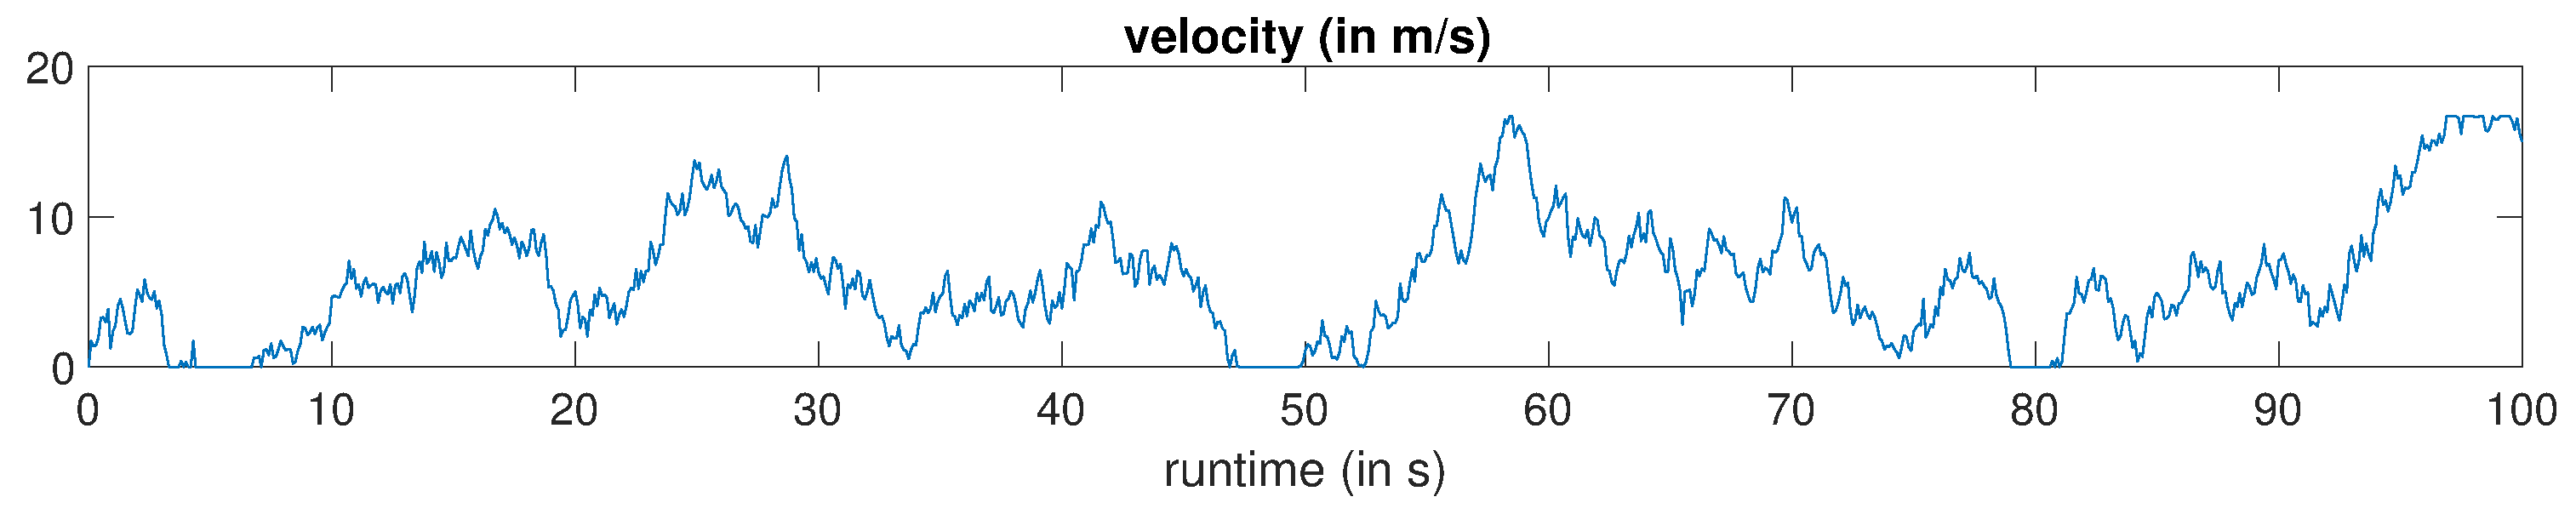
\includegraphics[width=0.95\textwidth]{images/AR1process}
	\caption{Example of a leading trajectory based on the parametrized AR1 process used to train the RL agent}
	\label{fig:AR1process}
\end{figure}
%
%\begin{figure}
%	\centering
%	\includegraphics[width=0.95\textwidth]{images/Training}
%	\caption{RL training process, one episode contains 500
%		steps. Shown are the reward values of the individual
%		episodes (blue) and a 30-step asymmetric moving average.}
%	\label{fig:training}
%\end{figure}
%
%


One \martin{training} episode has a simulation time of \unit[50]{s}.  With a step size of
$d=\unit[100]{ms}$, this results in an episode length of $500$
steps. The initial speeds of the following and leading vehicles are
randomly set in the range $[0,v\sub{des}]$ and $[0,v_{l,\text{des}}]$,
respectively. The initial space gap between both is set to \unit[120]{m}. 

\subsection{Model training}
Both neural networks, critic and Actor, are feed-forward neural networks with two layers of hidden neurons, containing 32 neurons each (see Figure \ref{fig:MRL}). ReLU activation functions are used. We used the same Ornstein-Uhlenbeck model as we used for the Free-Driving Policy.
All DDPG parameters are presented in Table \ref{tab:DDPGparameters}.

Figure \ref{fig:TrainingReward} shows an example of the training
process, where the asymmetric moving average reward of the last 30
training episodes is plotted over training episodes. For the
Car-Following Policy, a maximum average reward has been reached after
approximately 8900 training episodes (marked in red). The training processes for both policies are quite unstable. As this is a known issue using the DDPG algorithm, we plan to use a more stable algorithm like the TD3 algorithm \citep{TD3}.    








\section{Validation}
\label{sec:validation}
The goal is not to minimize some error measure as in usual
calibration/validation but to check if the driving style is safe,
effective, and comfortable. The RL strategy is evaluated with respect to these metrics in different driving scenarios, described in the following.

\subsection{Response to an external leading vehicle speed profile}
The first scenario is designed in order to evaluate the transition between free driving and car-following as well as the follower's behavior in safety-critical situations. 
Figure \ref{fig:manipulatedLeader} shows a driving scenario with an
artificial external profile for the leading vehicle speed. The initial
gap between 
follower and leader is 200 meters \martin{referring} to a free driving
scenario. The follower accelerates with $a\sub{max} = \unit[2]{m/s^2}$ until
the desired speed $v\sub{des} = \unit[15]{m/s} $ is reached and approaches
the standing leading vehicle. When the gap between both drops below 
\martin{\unit[70]{m}},
the follower starts to decelerate with a maximum
  deceleration of approximately $b_{\rm
  comf} = \unit[2]{m/s^2}$ (transition between free driving and car-following)
and comes to a standstill with a final gap of approximately 
$g\sub{min} = \unit[2]{m}$. Afterwards ($t=\unit[30]{s}$),  the leading vehicle accelerates to a speed
that is below the desired speed of the follower before performing a
maximum braking maneuver ($a=\unit[-9]{m/s^2}$) to a full stop ($t=\unit[46]{s}$). At the time of the start of the
  emergency braking, the follower has nearly reached a steady
  following mode at the desired space gap $g=s_0+v_l T$. While this
  gap makes it impossible to keep the deceleration in the comfortable
  range without a rear-end collision, the follower makes the best of
  the situation by braking smoothly with a maximum deceleration of $-a
  \approx \unit[5]{m/s^2}$.  The transition between different
accelerations happens in a comfortable way reducing the resulting
jerk. Only at the beginning ($t=\unit[46]{s}$) where the situation is
really critical, the jerk $\text{d}a/\text{d}t$ exceeds the comfortable range 
$\pm \unit[1.5]{m/s^3}$. Afterwards, the leader performs a series of
non-critical acceleration and deceleration maneuvers and the follower
tries to follow the leader at the speed dependent desired space gap
$g_0+v_lT$ while simultaneously smoothing the leader's speed profile. After the leaders speed exceeds the desired speed of the follower at $t=\unit[88]{s}$ (transition between car-following and free driving), the follower keeps the desired speed $v\sub{des} = \unit[15]{m/s} $.



\begin{figure}
	\centering
	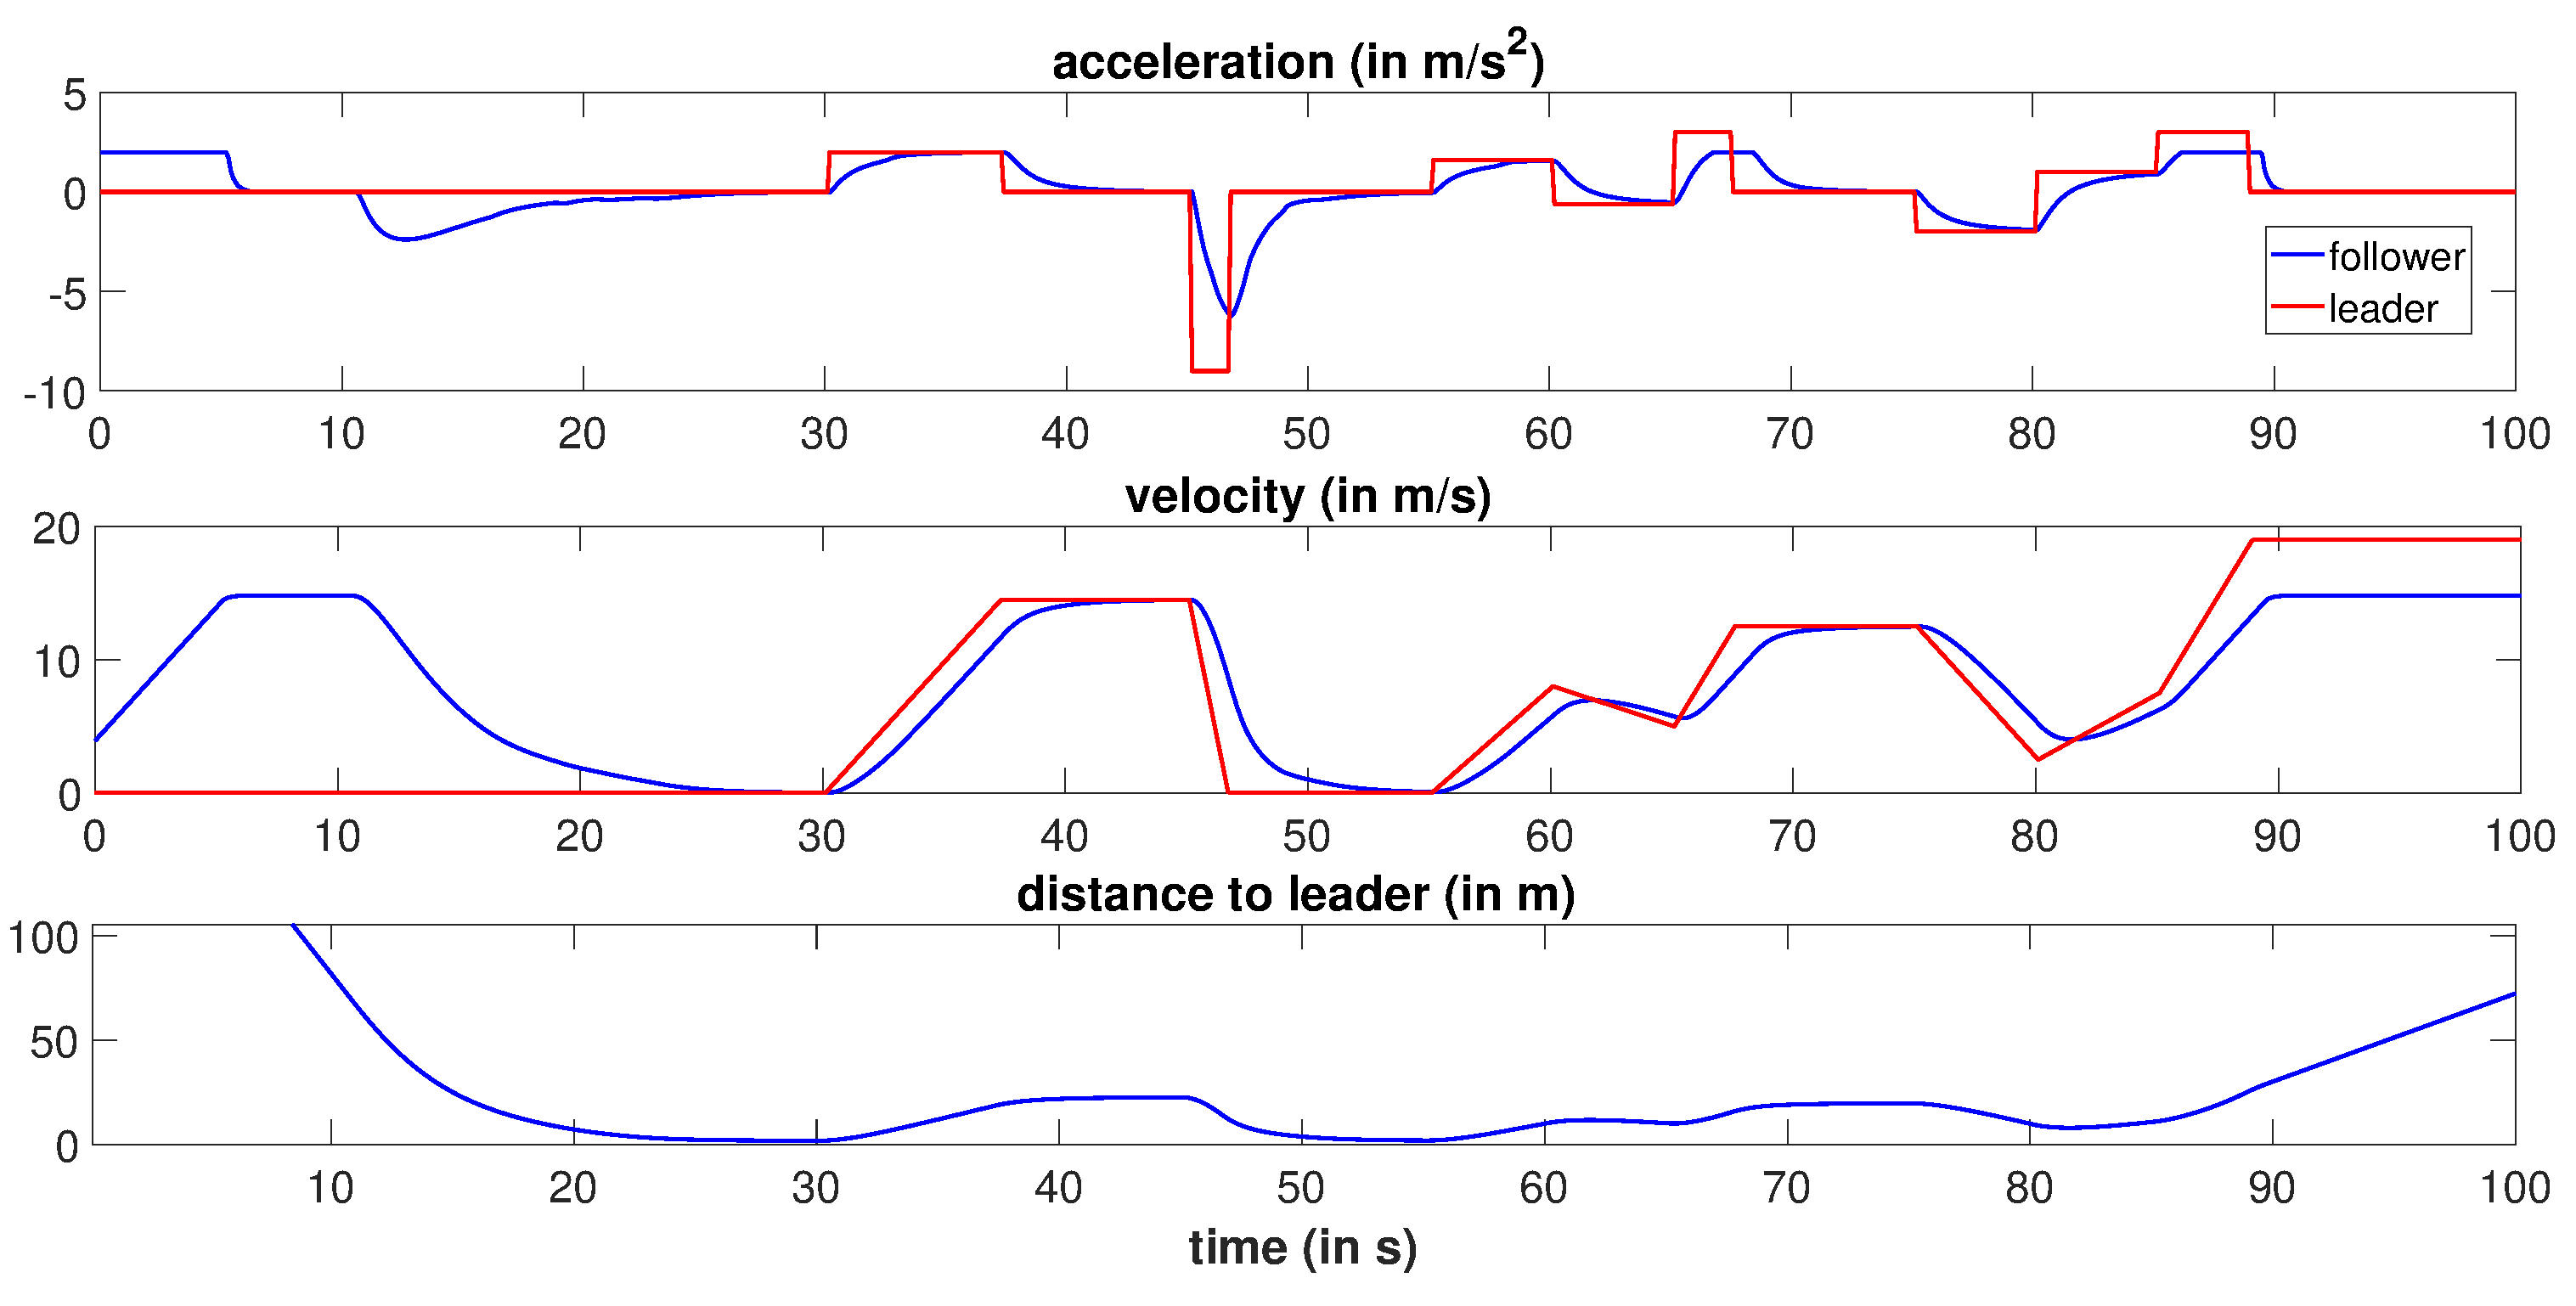
\includegraphics[width=0.95\textwidth]{images/manipulatedLeader.eps}
	\caption{Response to an external leading vehicle speed
          profile.}
	\label{fig:manipulatedLeader}
\end{figure}

\begin{figure}
	\centering
	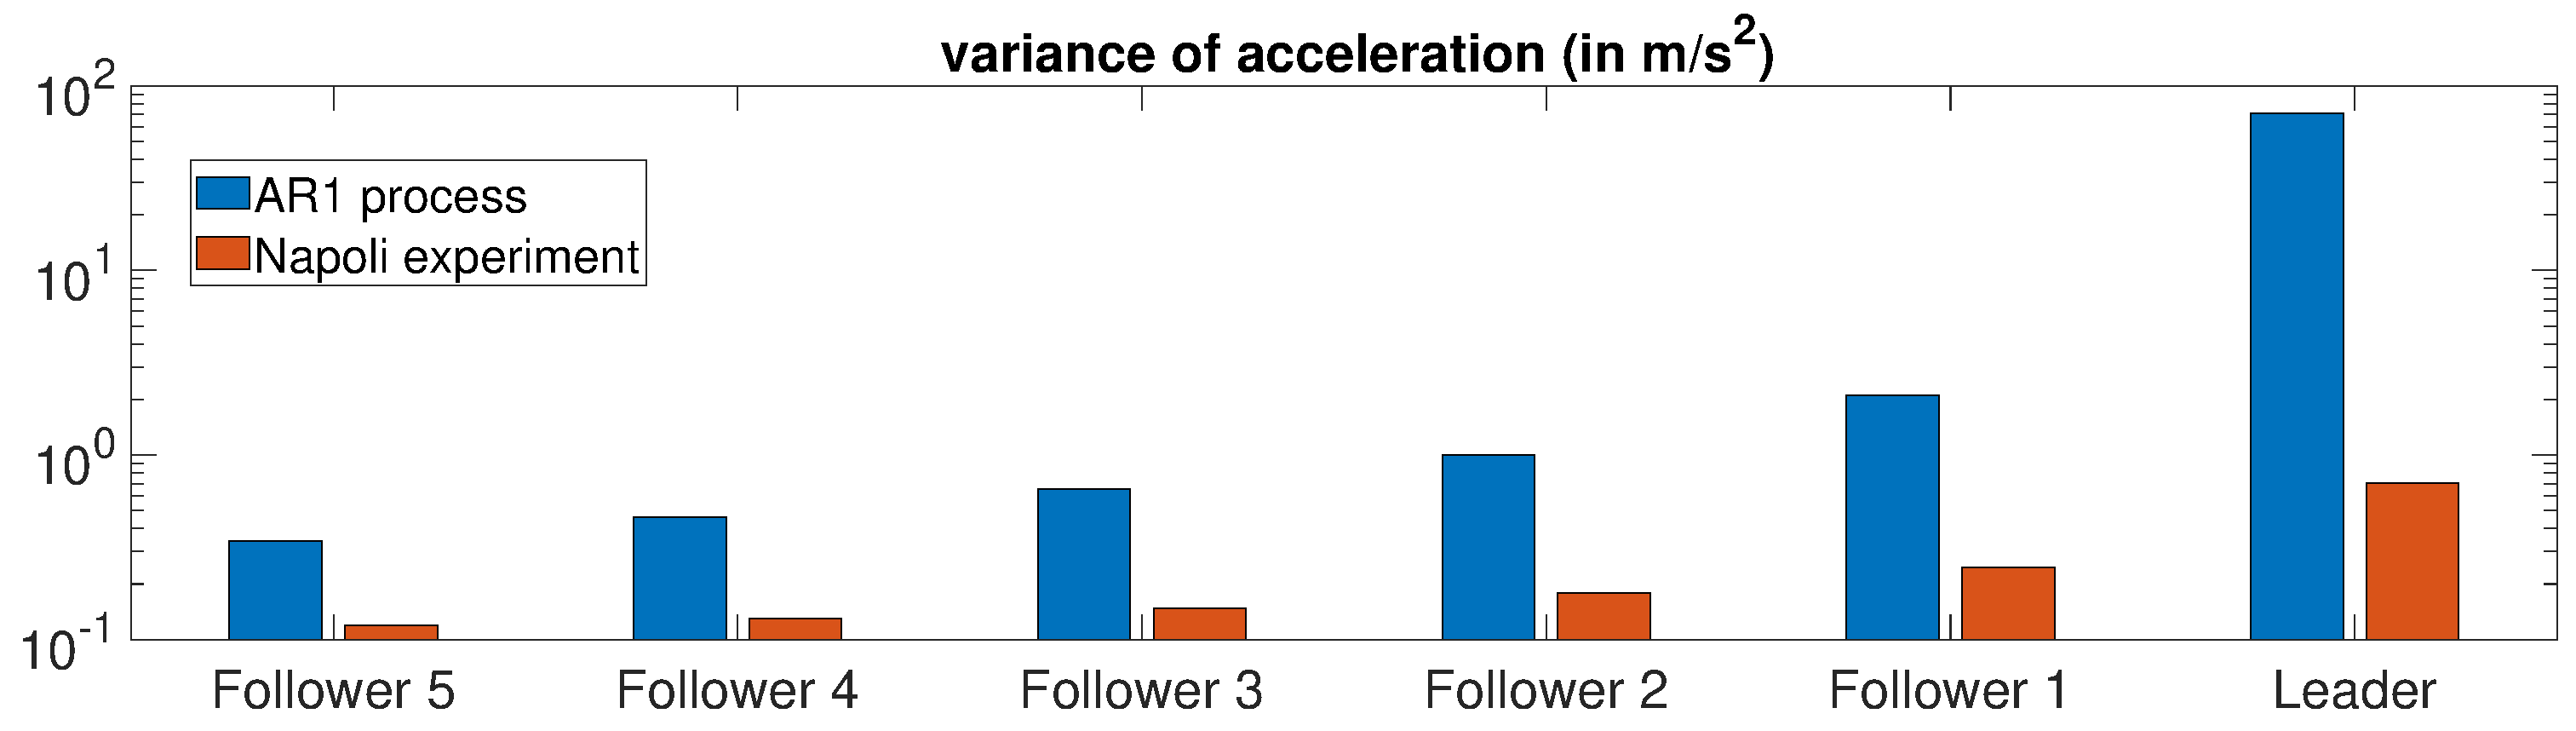
\includegraphics[width=0.95\textwidth]{images/VarAccComp}
	\caption{Comparison of the acceleration variance between
          leader and follower for a leader controlled by AR(1) (blue
          bars) and the leading vehicle of the Napoli experiment
          (red).}
	\label{fig:VarAccComp}
\end{figure}






\subsection{String stability}
\label{sec:stringStability}
The second validation scenario, shown in Figure
\ref{fig:AR1Kolonne}, consists of a leader based on the AR(1) process
that is
followed by five vehicles, each controlled by the trained RL
agent. The results show that traffic oscillations can effectively be
dampened with a sequence of trained followers, even if the leader
shows large outliers in acceleration. Figure \ref{fig:VarAccComp}
illustrates the difference of accelerations between leader and the
followers (blue bars). The last follower shows the lowest variance of
acceleration \martin{demonstrating} the ability of the RL agent to
flatten the speed profile, to dampen oscillations, and thus to increase
comfort and reduce fuel consumption and emissions.   


\begin{figure}
	\centering
	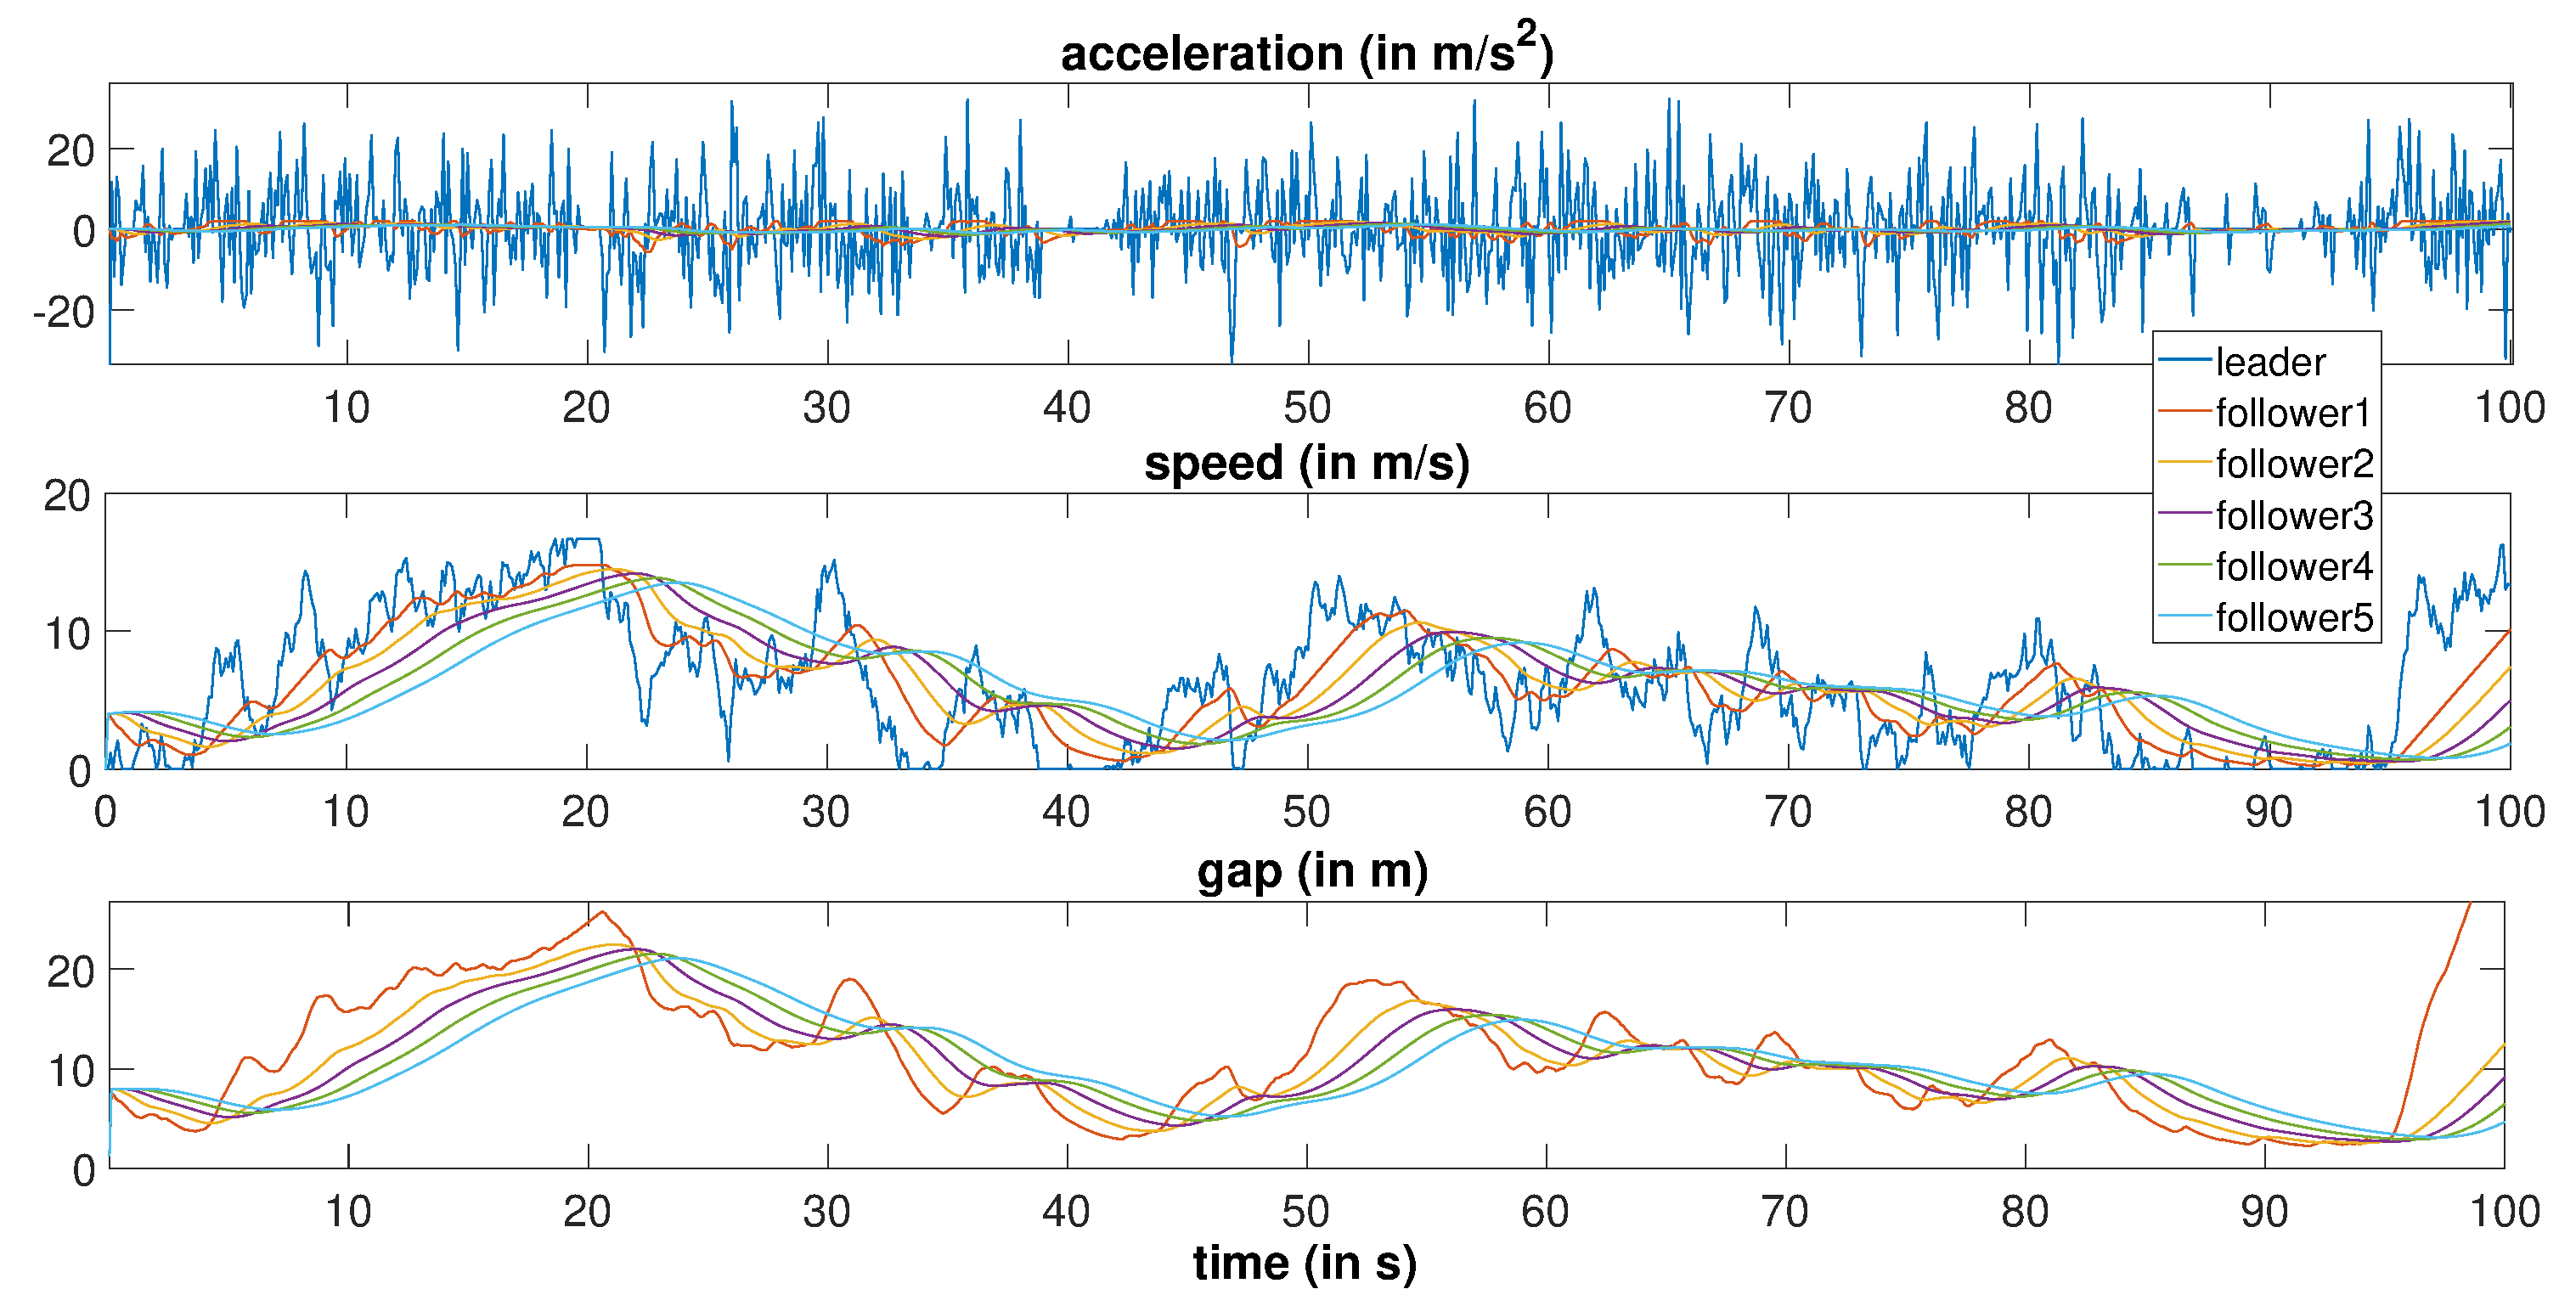
\includegraphics[width=0.95\textwidth]{images/AR1Kolonne}
	\caption{Response to a leader trajectory based on a AR(1) process}
	\label{fig:AR1Kolonne}
\end{figure}


\subsection{Response to a real leader trajectory}

In a further scenario, the abilities of the RL strategy are evaluated
with a real leader trajectory (Fig.~\ref{fig:PunzoKolonne}). This
trajectory comes from \martin{the platoon driving experiments of
  \cite{punzo2005nonstationary} on urban and peripheral arterials in Napoli}
where high-precision distance data between the platoon
vehicles were obtained. Similar to the experiment from
Section~\ref{sec:stringStability}, string stability and the reduction
of  the acceleration variance, shown by the red bars in Figure
\ref{fig:VarAccComp}, is demonstrated. At time $t = \unit[140]{s}$ the leader
stands still and it can be observed that all following vehicles are
keeping the minimum distance $g\sub{min}$ to the leader.  


\begin{figure}
	\centering
	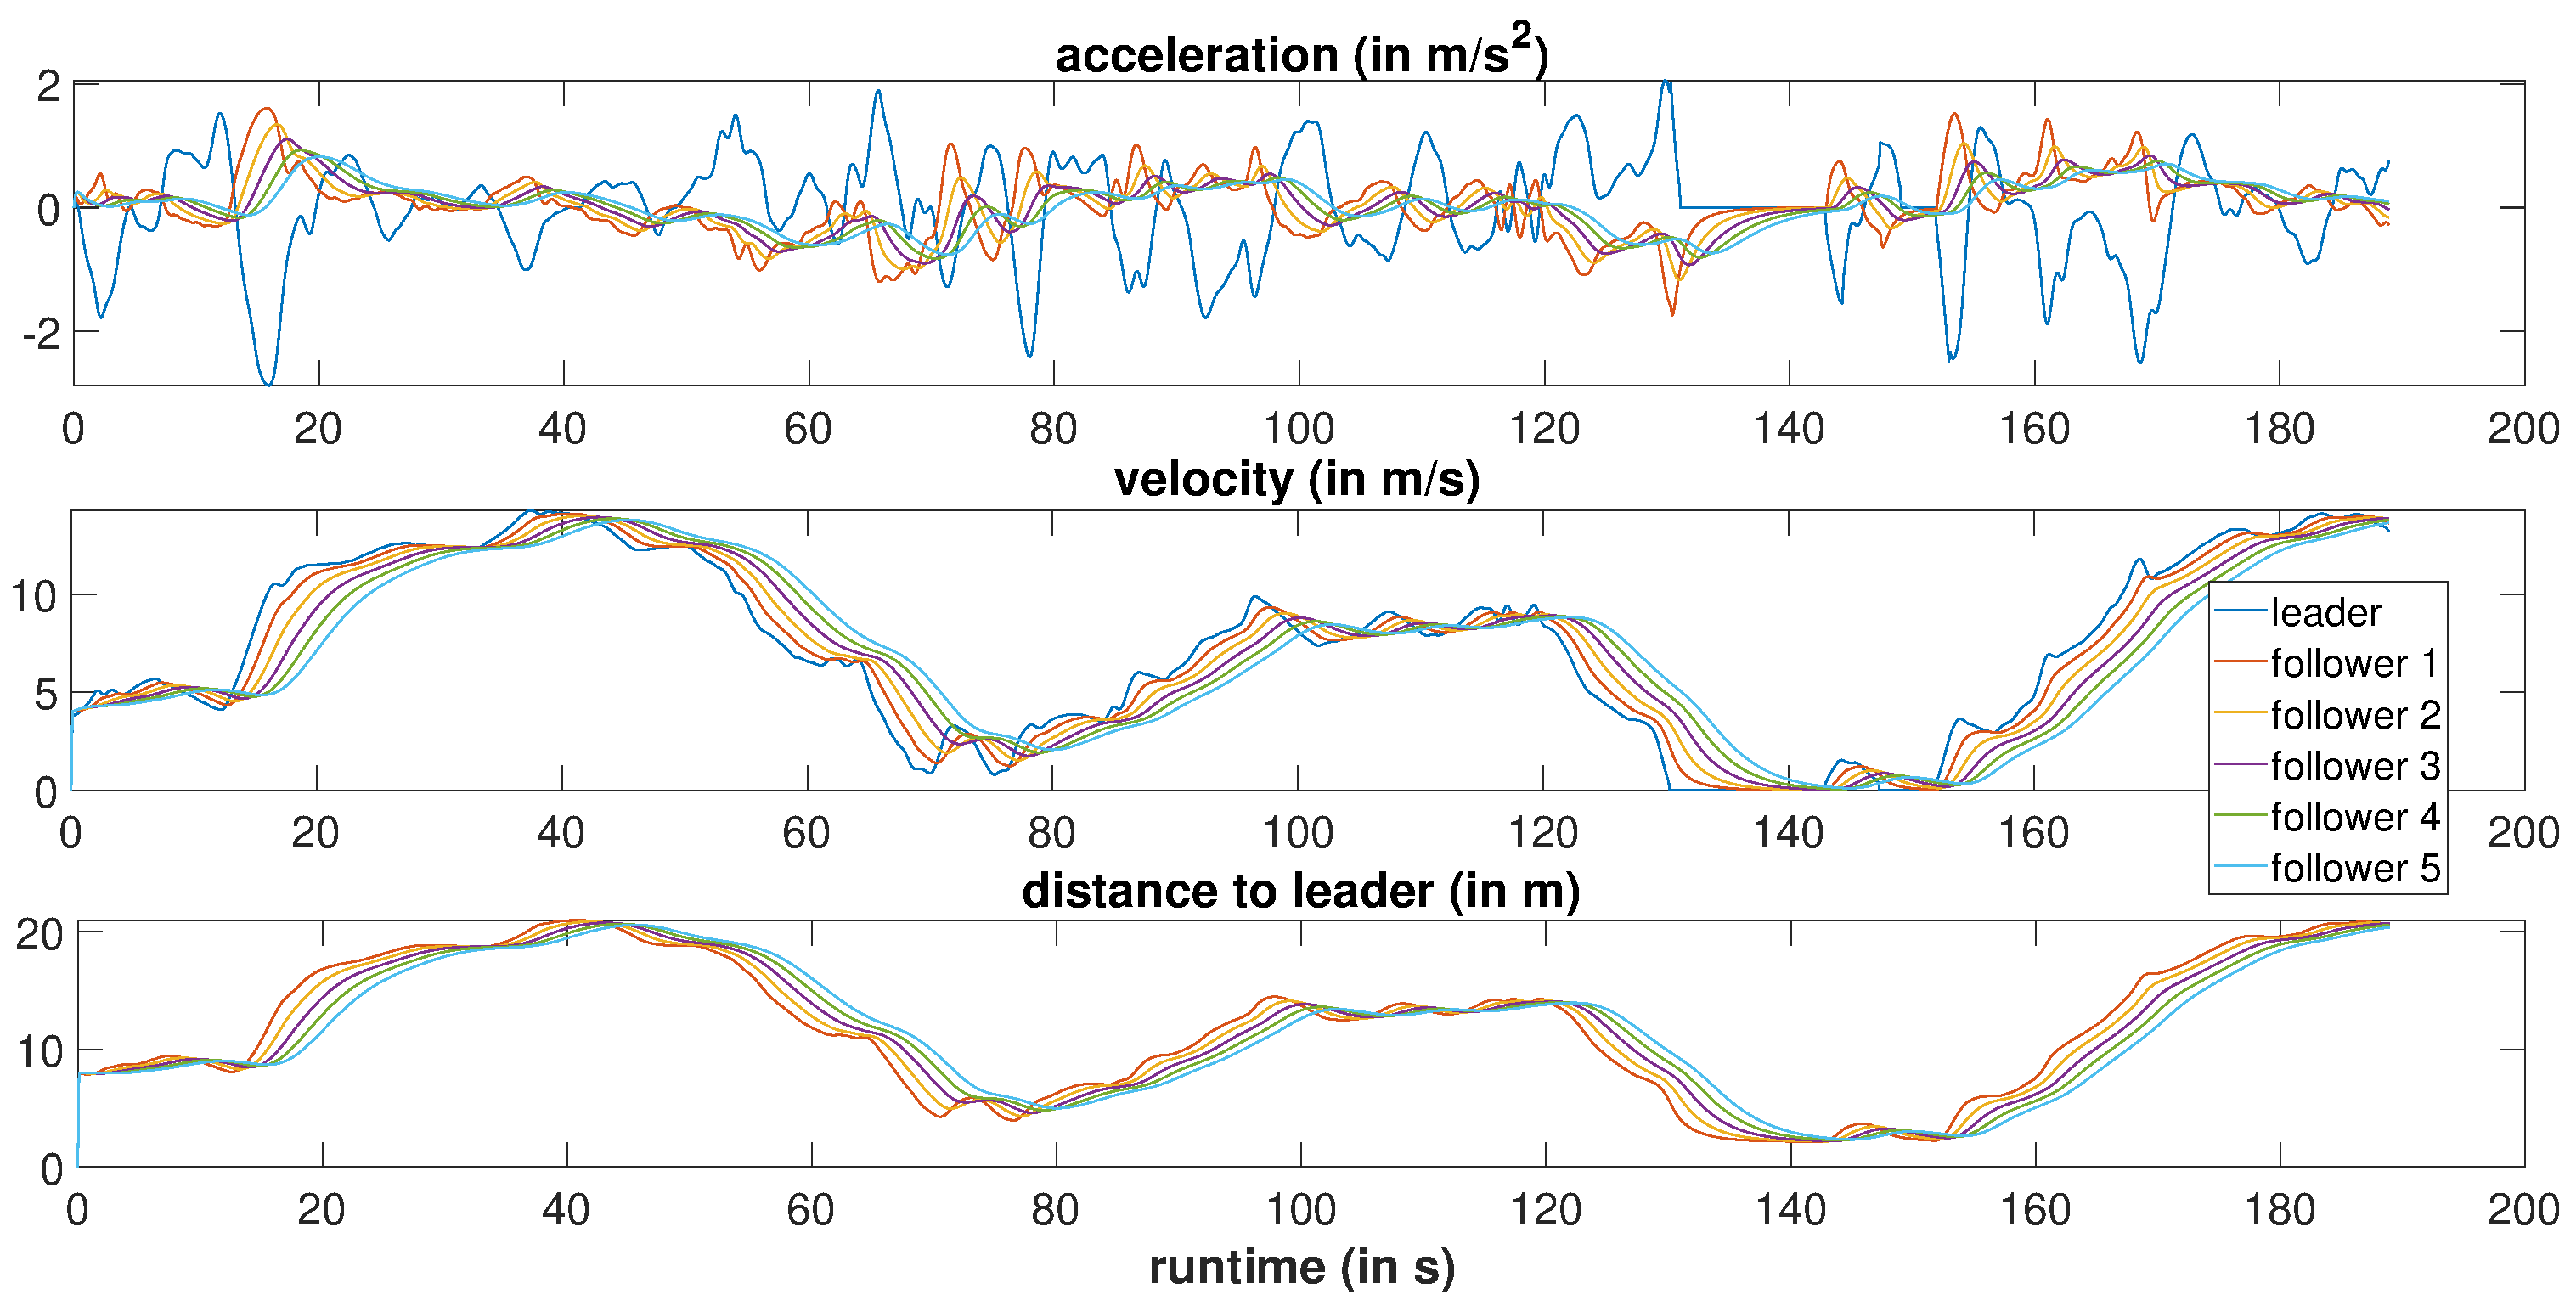
\includegraphics[width=0.95\textwidth]{images/PunzoKolonne}
	\caption{Response to a real leader trajectory}
	\label{fig:PunzoKolonne}
\end{figure}


\subsection{Response of different driver characteristics}
\label{sec:differentT}

As mentioned in Section \ref{rewardFunctionFollow}, different driving styles
can be achieved by adjusting the parameters of the reward
function. Three RL agents has been trained on a reward function, that
differs in the desired time gap $T$ between following and
leading vehicle ($T_{1} = 1.0s$, $T_{2} = 1.5s$, 
$T_{3} =2.0s$). Figure \ref{fig:differentT} shows the result of these agents,
following the real leader trajectory from Napoli. It can be observed,
that a lower value for $T$ results in closer driving to the
leader which can be considered as a more ``aggressive''
driving style. \martinc{It would be instructive to have a time series
  plot of the actual time gap $g/v$ or $(g-g_0)/v$ (restricted to
  values $<2T$). For the IDM, these
  are somewhat higher in steady state: Analytical expression 
$T_e(v):=(g_e(v)-g_0)/v=T/\sqrt{1-(v/v_0)^4}$, for the IDM+ $T_e(v)=T$
  for $v<v_0$}
Since this also means that there are less options in
increasing driving comfort without affecting safety, the follower's
accelerations and decelerations are higher than that of the more
conservative RL agent~3 although the relative
weighting $w\sub{jerk}/w\sub{gap}$ of the safety and comfort aspects in Eq.~\eqref{rt1} and \eqref{rt2} has not been
changed. Still, when simulating platoons of the three RL
  agents in any order, the accelerations and jerks decrease along the
  platoon.

\begin{figure}
	\centering
	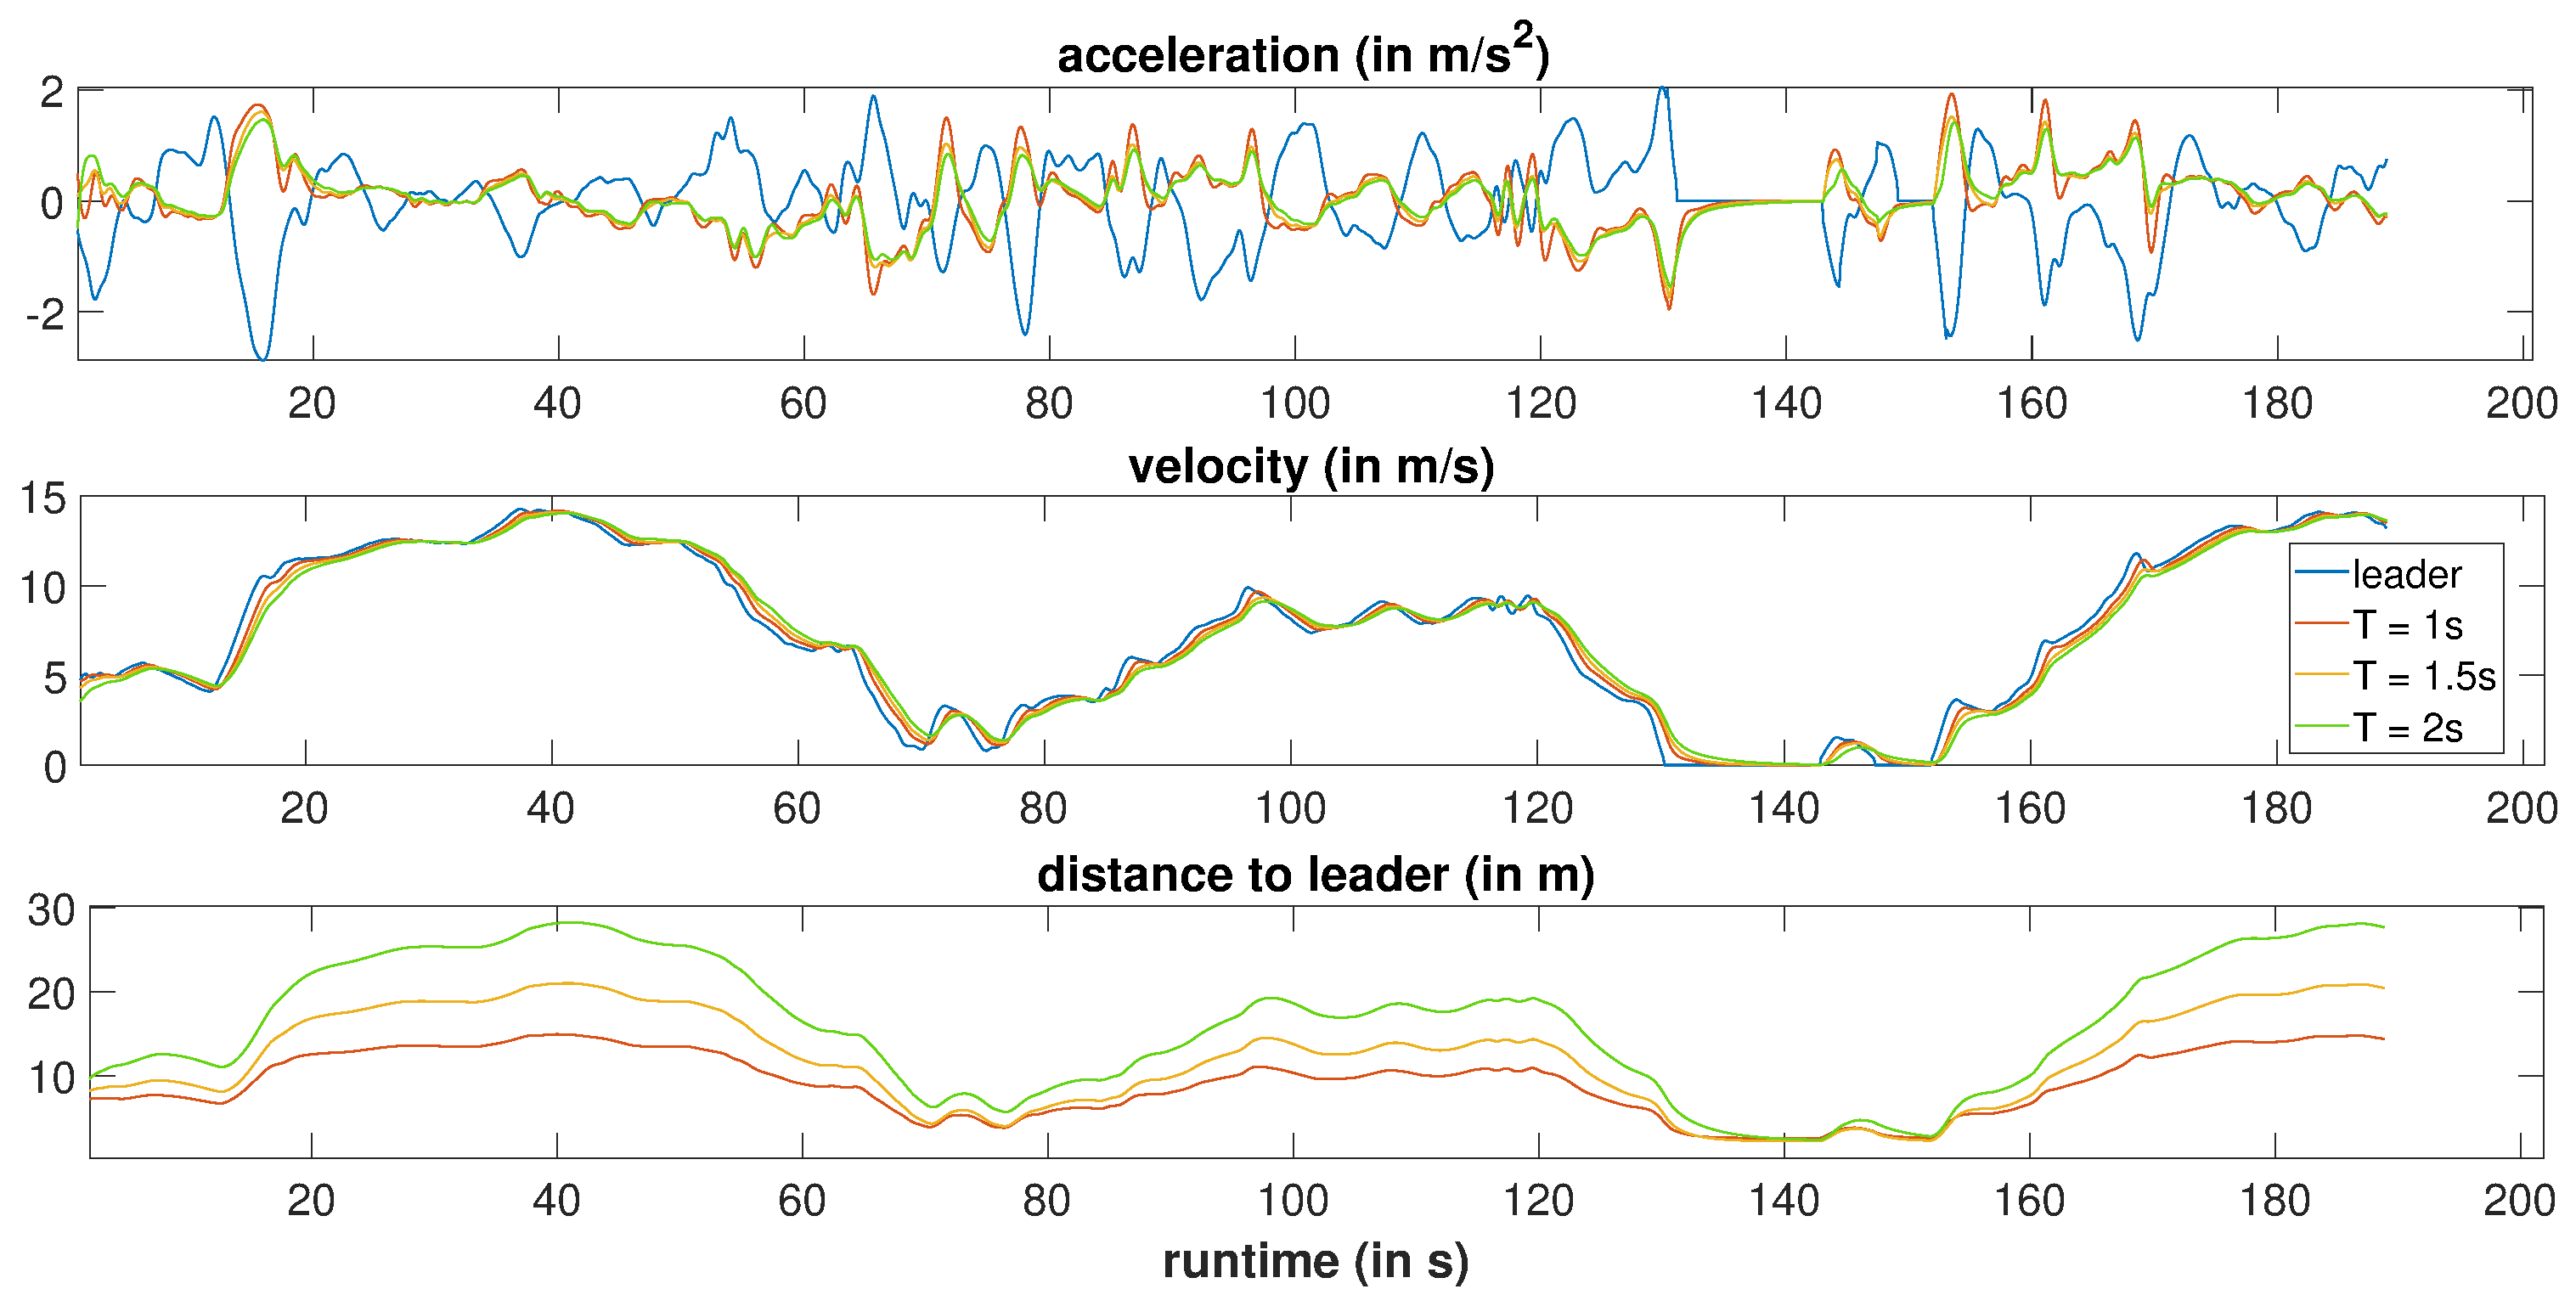
\includegraphics[width=0.95\textwidth]{images/differentT}
	\caption{Impact of differently parametrized RL agents
          on the driving behavior }
	\label{fig:differentT}
\end{figure}


\subsection{Cross validation with the Intelligent Driver Model}
\label{sec:crossValIDM}
To compare the performance of the RL agent with that of
classical car-following models, we chose the commonly used
Intelligent-Driver Model (IDM) of \cite{Opus} whose acceleration is given
by 
\begin{equation}
\label{eq:IDM}
\martin{\dv{v}{t}}=a\sub{max}\left(1-\left(\frac{v}{v\sub{des}}\right)^{4}-\left(\frac{s^{*}\left(v, \martin{v_l}\right)}{g}\right)^{2}\right),
\end{equation}
with
\begin{equation}
\label{eq:IDMsstar}
s^{*}\left(v, v_l\right)=g\sub{min}+\max \left(0,vT+\frac{v(v-v_l)}{2 \sqrt{a\sub{max} b\sub{comf}}}\right).
\end{equation}
Notice that the IDM parameters desired
speed $v\sub{des}$, minimum gap $g\sub{min}$, time gap $T$, maximum
acceleration $a\sub{max}$, and
comfortable deceleration $b\sub{comf}$ are a subset of that of the RL reward
function. 

First, we calibrate the IDM on the Napoli data set by
minimizing the sum of squares of the relative gap error,
$\mathrm{SSE}(\ln g)$, of the first follower with respect to the
data (cf. Table~\ref{tab:IDMparameters}). The same parameters are also
assumed for the reward function of the RL agent before it was trained
on the artificial AR(1) generated leader speed profile. Notice that the RL agent used the Napoli data only
indirectly by parameterizing its reward function.

\begin{table}
	\caption{IDM parameters calibrated to the Napoli
            data and also used for the reward function of the RL agent}
	\label{tab:IDMparameters} 
	\begin{center}
		\begin{tabular}{ p{0.14\textwidth} |p{0.1\textwidth}  } 
		Parameter & Value   \\ \hline
			$T$ & $\unit[0.83]{s}$\\
			$g\sub{min}$ & $\unit[4.90]{m}$\\
			$a\sub{max}$ & $\unit[4.32]{m/s^2}$\\
			$b\sub{comf}$ & $\unit[2.34]{ m/s^2}$\\
			$v\sub{des}$ & $\unit[33.73]{m/s}$
			
		\end{tabular}
	\end{center}
\end{table}

Figure \ref{fig:IDMvsRL} shows the results for \martin{(i)} the RL
agent, calibrated on the real follower data (red lines), (ii) the IDM,
calibrated on the same follower data (amber), and (iii) the real
follower of the Napoli experiment (red). To \martin{compare} the
performance for both approaches, the respective objective functions
have been computed. The objective function of the RL agent corresponds
to the reward function, while the goodness-of-fit function
\martin{$\mathrm{SSE}(\ln g)$} defines the objective function of the
IDM. \martin{Furthermore, we cross-compared the values by calculating the
reward function for the IDM and $\mathrm{SSE}(\ln g)$ for the RL model. All
values are shown in Table \ref{tab:objectiveFunc}. 
As expected, the RL agent performs better than the IDM relative to the
  reward function used for its learning. It is remarkable, however, 
 that the RL model also outperforms the IDM relative to the
 goodness-of-fit function which has been used only indirectly by
 parameterizing its reward function.}

\begin{figure}
	
	\centering
	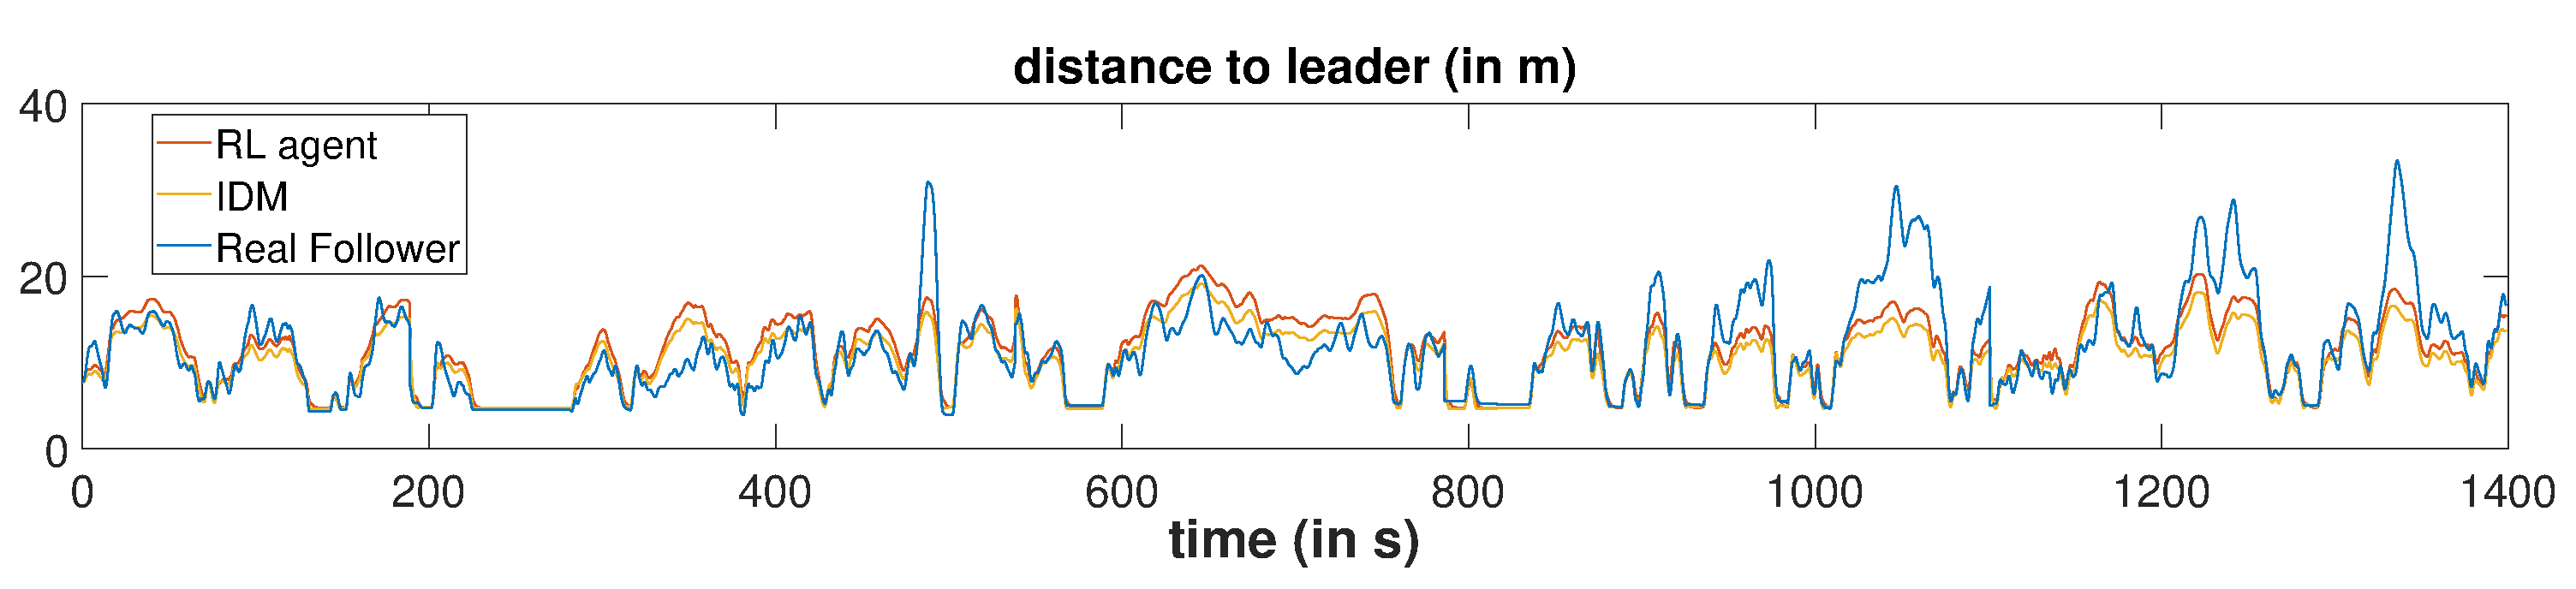
\includegraphics[width=0.95\textwidth]{images/IDMvsRL_dist}
	\caption{Comparison between IDM and RL agent, calibrated on the same set of parameters}
	\label{fig:IDMvsRL}
\end{figure}

\begin{table}
	\caption{Comparison between calibrated RL agent and IDM for
          accumulated Reward and Goodness-of-Fit Function $\mathrm{SSE}(\ln g)$} 
	\label{tab:objectiveFunc} 
	\begin{center}
		\begin{tabular}{p{0.3\textwidth} | p{0.2\textwidth} p{0.2\textwidth}  } 
			& RL agent & IDM   \\ \hline
			$\mathrm{SSE}(\ln g)$ & $389.10$ &  $418.05$	\\
			Accumulated Reward &  $6.86 \times 10^3$   & $6.73\times 10^3$
			
		\end{tabular}
	\end{center}
\end{table}

\subsection{Time-to-collision comparison with the Intelligent Driver Model}

An important safety measure for car-following models is the
time-to-collision (TTC). Again we took leading trajectories coming
from platoon driving experiments in Napoli to conduct a TTC
analysis. We simulated 15 different leaders from those experiments,
once followed by an RL agent and the other time by an IDM vehicle (Sect. \ref{sec:crossValIDM}). Both
followers are parametrized according to the default parameters of Table
\ref{tab:agentParameters}. Figure \ref{fig:DistributionTTC} shows the
distribution of TTC for all 15 experiments. The TTC has been evaluated
at each simulation time step. The lower TTC bound for the RL agent is
\unit[1.99]{s}, while the one for the IDM vehicle is
\unit[2.04]{s}. But except for some values around TTC = \unit[2]{s}, the TTC values of the RL agent show to be higher than those of the IDM.

The difference in driving behavior is further
evaluated by focusing on a single leader-follower experiment, shown in
Figure \ref{fig:TTC_CaseStudy}, where the situation with the lowest TTC for the RL agent is marked green. In this situation, the leader brakes to a standstill with a 
quite high deceleration of $b = \unit[6]{m/s^2}$. The reason for the slight
difference in TTC between IDM and RL agent lies in the fact, that the
IDM keeps a slightly higher gap to the leader most of the time,
which simply reflects a more defensive driving style. 

\begin{figure}	
	\centering
	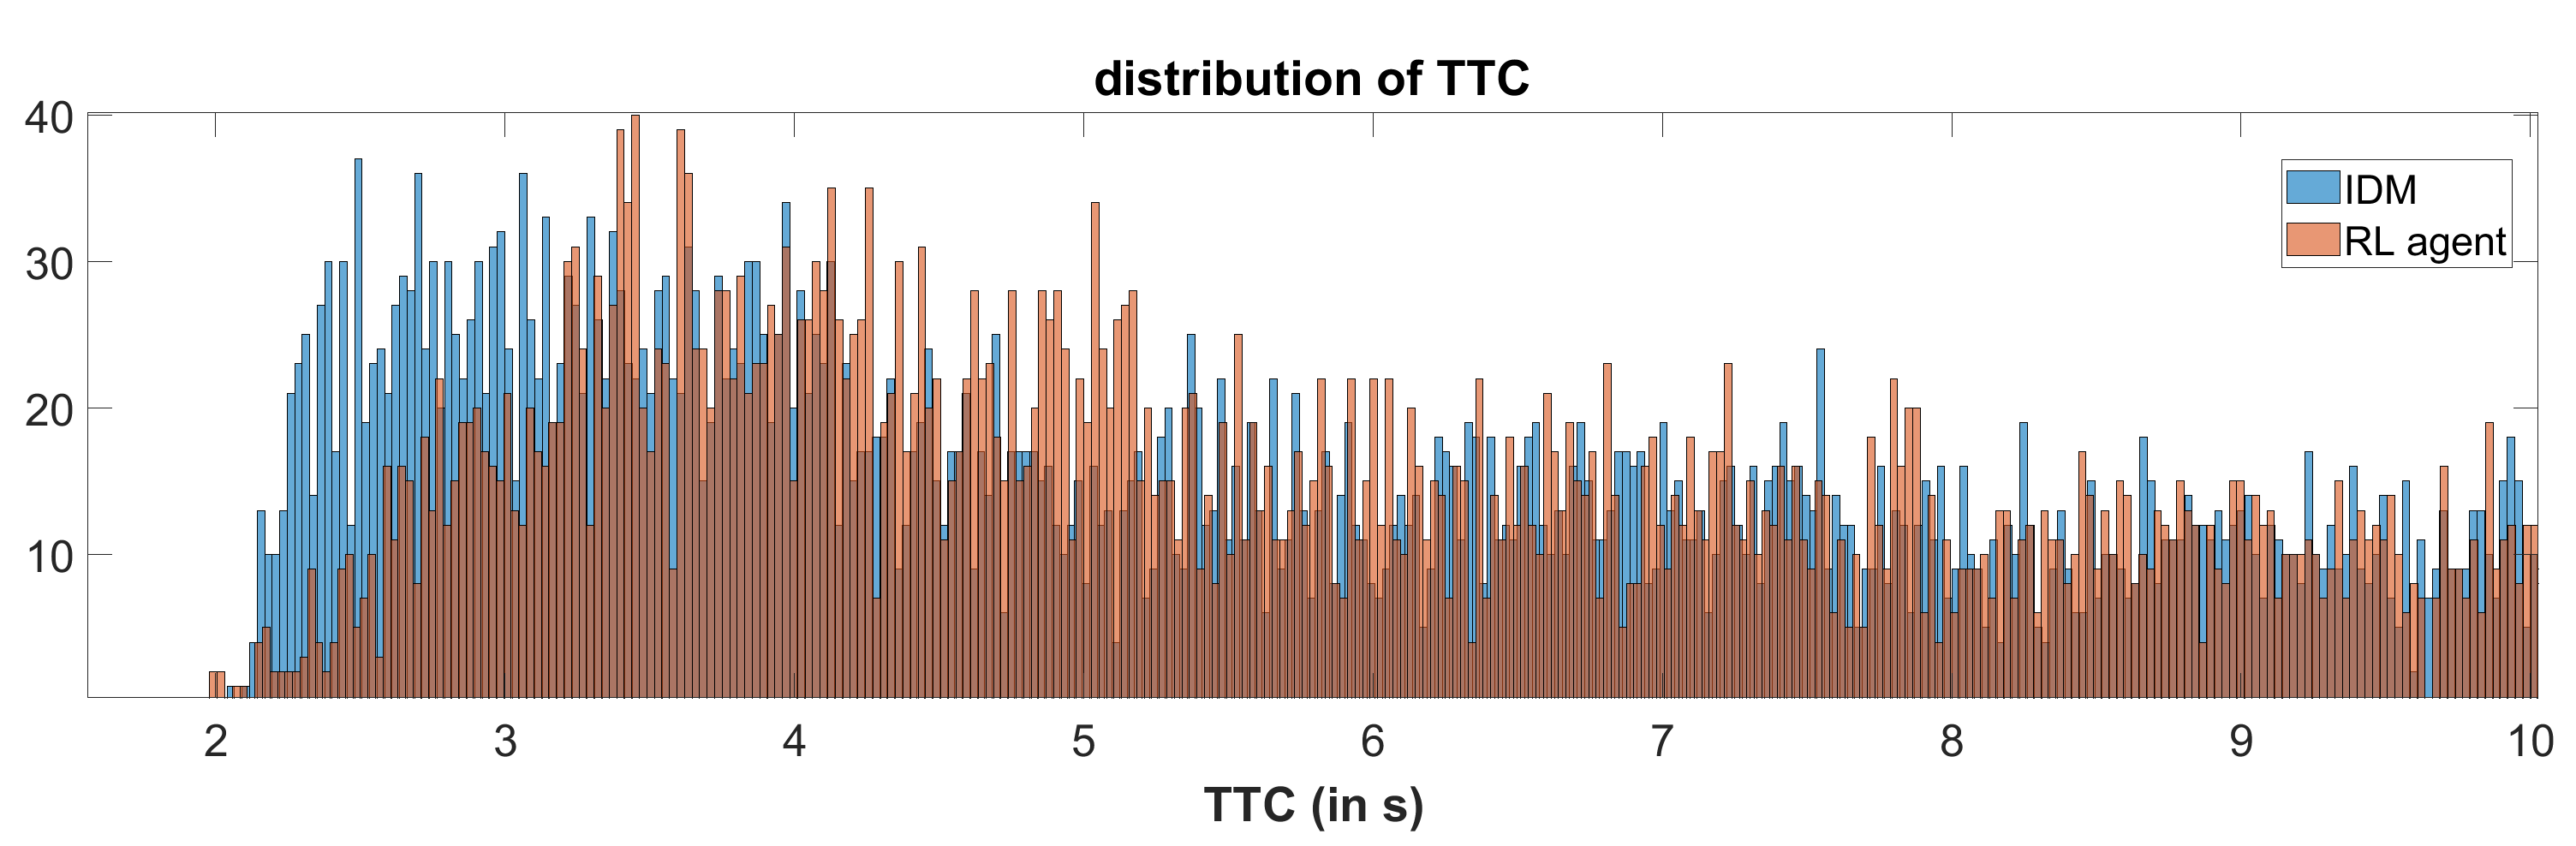
\includegraphics[width=0.95\textwidth]{images/TTC}
	\caption{Distribution of time-to-collision (TTC) for IDM and RL agent in different experiments based on real leader trajectories}
	\label{fig:DistributionTTC}
\end{figure}

\begin{figure}	
	\centering
	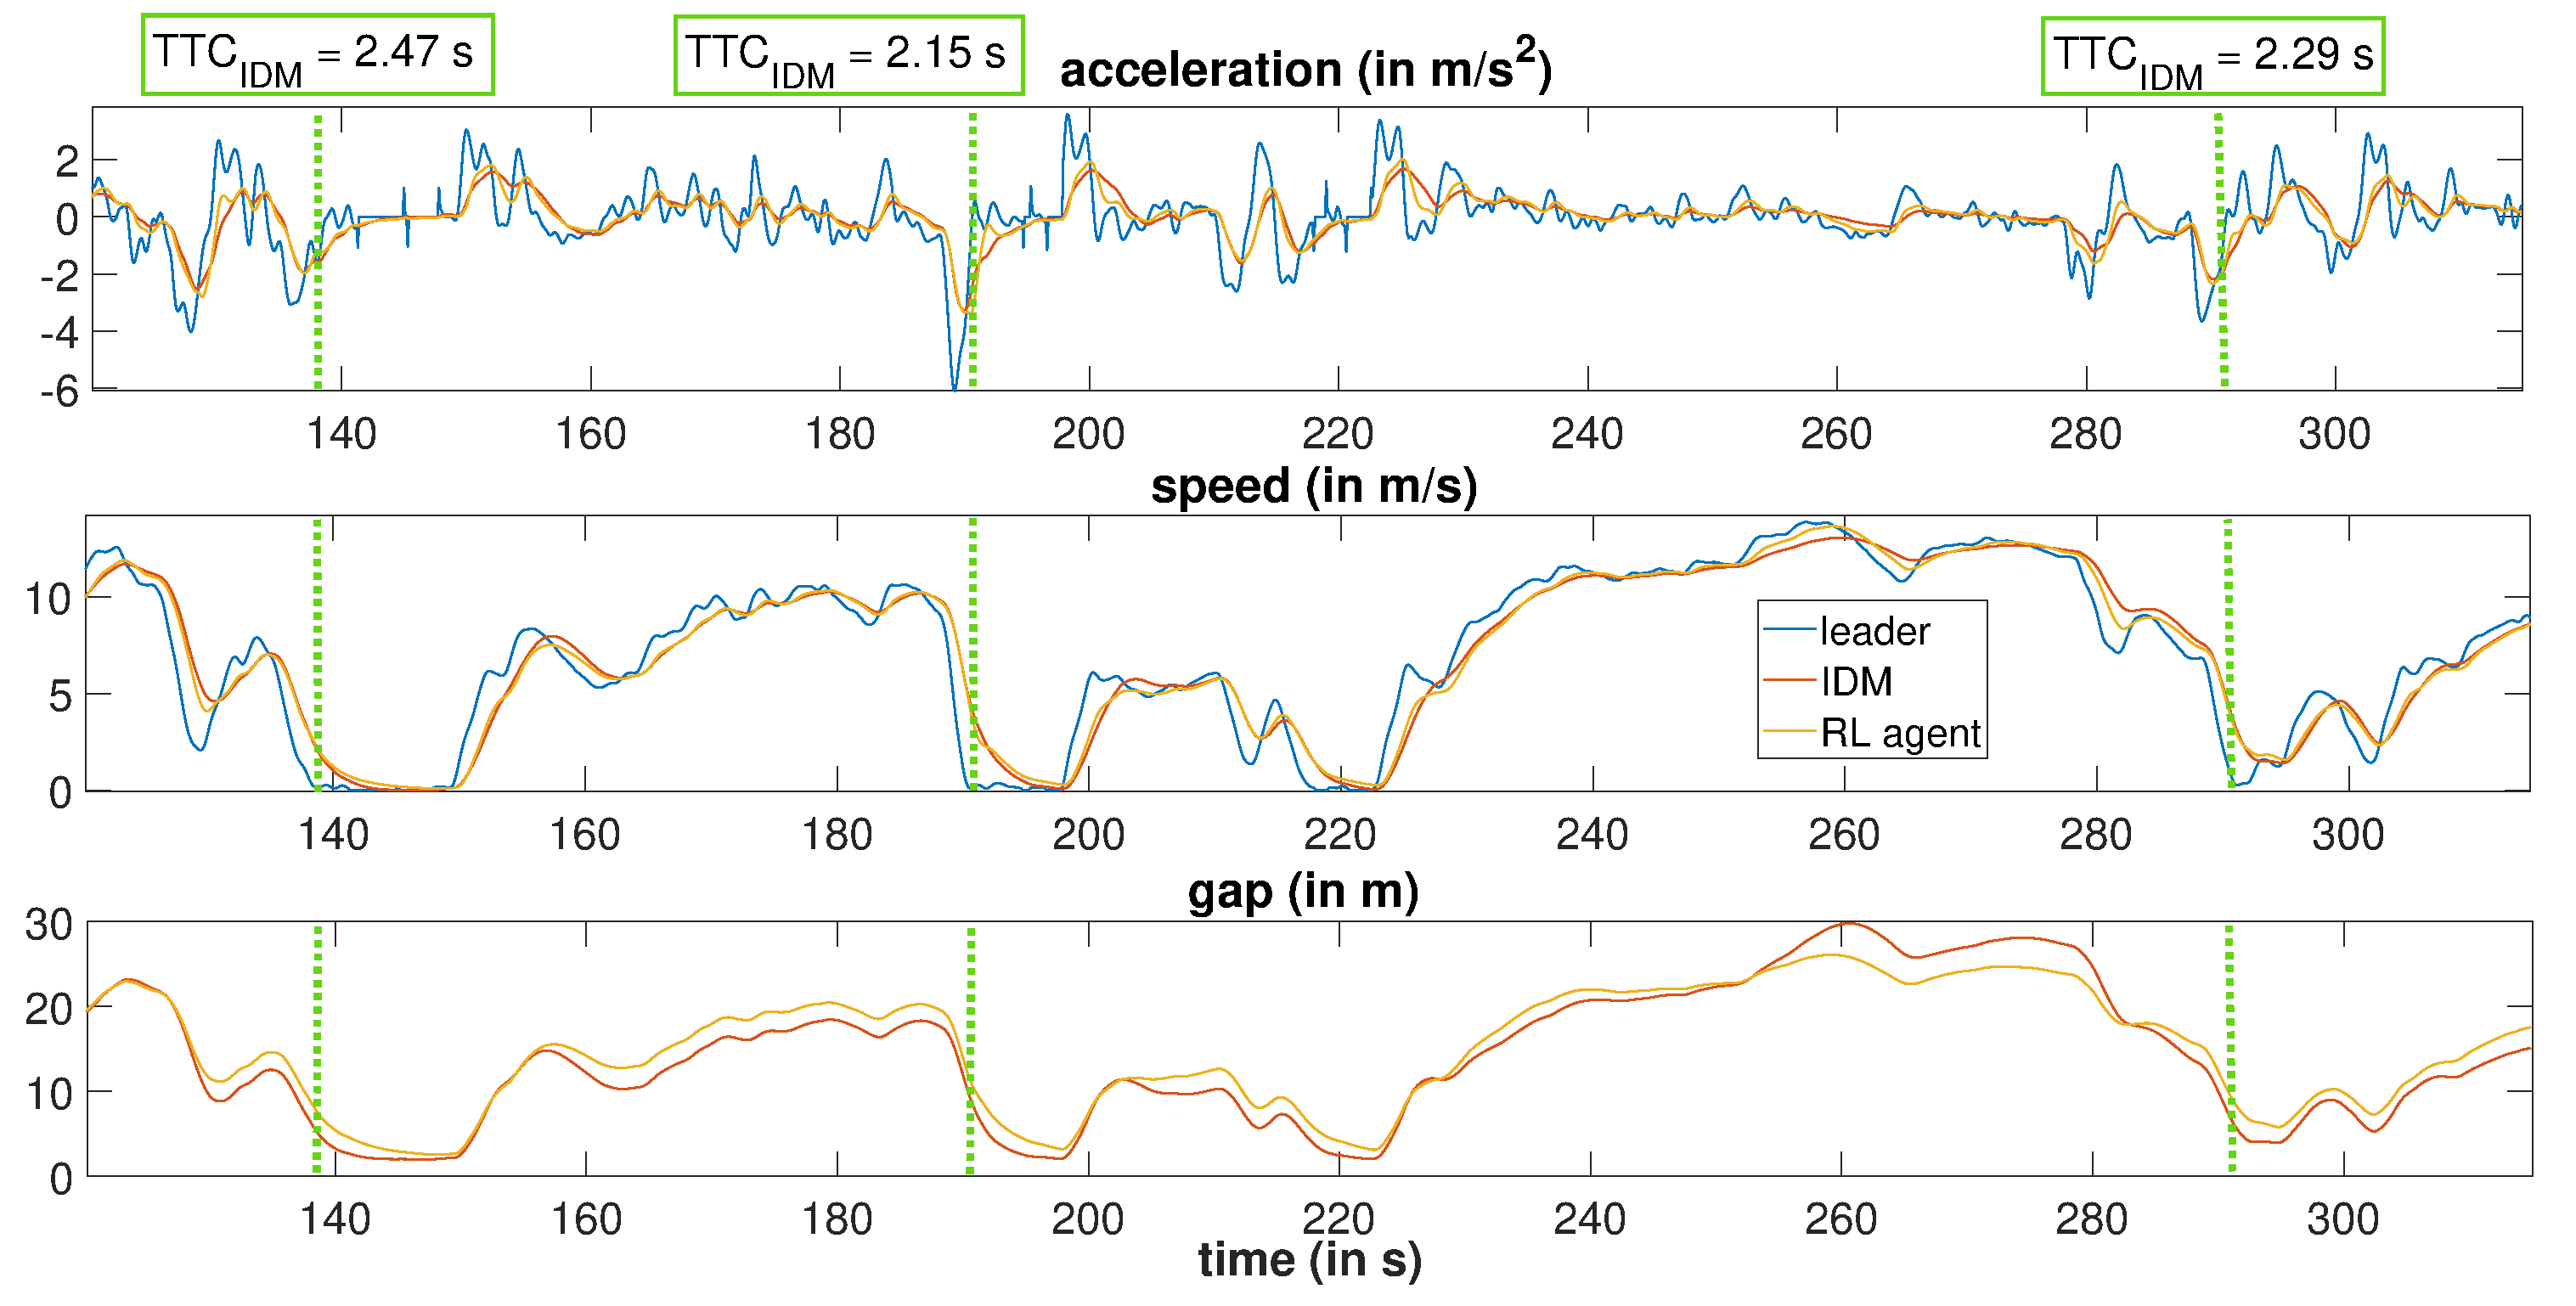
\includegraphics[width=0.95\textwidth]{images/TTC_CaseStudy}
	\caption{Response of an IDM and RL agent on a real trajectory. Safety-critical situations where the TTC of the IDM drops below \unit[2.5]{s} are marked in green.}
	\label{fig:TTC_CaseStudy}
\end{figure}

\section{Conclusion/Discussion}
\label{sec:conclusion}
This study presented a novel car-following model based on
\martin{Deep Reinforcement Learning}. \martinc{Die Conclusion wird
  bisweilen separat gelesen, so besser (wie immer im Abstract) keine
  Abk\"urzungen verwenden, au\3er die allergebr\"auchlichsten} The
proposed model considers free driving, car-following, as well as the
transition between both in a way, that approaching the leading vehicle
is smooth and comfortable. We used an approach called Modularized
Reinforcement Learning (\cite{MRL}) to decompose the multi-goal
problem into two subtasks. Two different RL policies have been
designed using the Deep Deterministic Policy Gradient algorithm. The
Free-Driving Policy \martin{aims to reach and not exceed a certain
desired speed.} The Car-Following Policy aims to keep a reasonable gap
to a leader vehicle \martin{and keep the traffic situation safe.} 

For each policy, we defined separate reward functions \martin{reflecting} traffic safety and comfort aspects. 
Different driver characteristics can be modeled by adjusting the parameter of the reward function.

The proposed model is trained on leading trajectories based on an
AR(1)-process. This leads to high generalization capabilities and a
model usage in a wider variety of traffic scenarios. \martin{Furthermore, the
supply of learning data is unlimited.}
For the evaluation of the trained agents, different traffic scenarios
\martin{based on both synthetic and
real trajectory data have been simulated, including situations that
bring the model} to its limits. 
In all cases, the car-following model proved to be accident-free and
comfortable. Further scenarios showed that traffic oscillations could
effectively be dampened with a sequence of trained followers, even if
the leader shows large outliers in acceleration.

\martin{Besides driving comfort, string stability, and safety,
  the efficiency of the resulting traffic flow is important,
  particularly, the fundamental diagram, the maximum flow through a
  bottleneck that can be 
  sustained and the outflow from a region of congested
  traffic. Furthermore, we have idealized the state dynamics by
  assuming that a vehicle can instantaneously take on the acceleration
  prescribed by the actor while the real control path is more
  complicated and non-negligible response times happen, particularly
  for positive accelerations. We expect that RL techniques play out
  their strengths in such more complex state dynamics. All this  will
  be investigate in a forthcoming paper.
}

\martin{
\subsection*{Acknowledgements}
We thank Vincenzo Punzo for making available to us the experimental
car-following data used in this paper. This work was funded by ...}
\martinc{Ostap: DFG oder andere funds nennen?}





\bibliography{RL_vehicles_references}

\end{document}
